\section[LDI]{Lagrangian Droplet Impingement}

% Section transition: 03_LAGRANGIAN_DROPLET_IMPINGEMENT
{\renewcommand{\iceImgX}{1.01}\renewcommand{\iceImgY}{0.22}%
\IceSectionDivider[height=0.98\H]{}{Lagrangian\\ Droplet Impingement}{FIGURES/SECTION_TRANSITION/dropletTrajectoriesChapelCon.png}}


\begin{frame}{Droplet Impingement: Collection Efficiency}
\vspace{0.08cm}

The droplet solver determines the \textbf{local water mass flux}
reaching the aircraft surface.

\vspace{0.08cm}
\begin{columns}[T,onlytextwidth]
\begin{column}{0.43\textwidth}
{\color{champsBlue}\bfseries Collection Efficiency}

\vspace{0.04cm}
\small
The ratio of local impinging water flux to the
freestream water flux:\par\vspace{0.05cm}
{\centering$\displaystyle\beta = \frac{\dot m_{\mathrm{imp}}}{\mathrm{LWC}\,U_\infty}$\par}

\vspace{0.1cm}
{\color{champsBlue}\bfseries Water Mass Flux}\par
Accounting for the cloud liquid water content
(LWC, in g/m$^3$):\par\vspace{0.05cm}
{\centering$\boxed{\dot m_{\mathrm{imp}}=\beta\,\mathrm{LWC}\,U_\infty}$\par}
\end{column}

\begin{column}{0.54\textwidth}
\centering
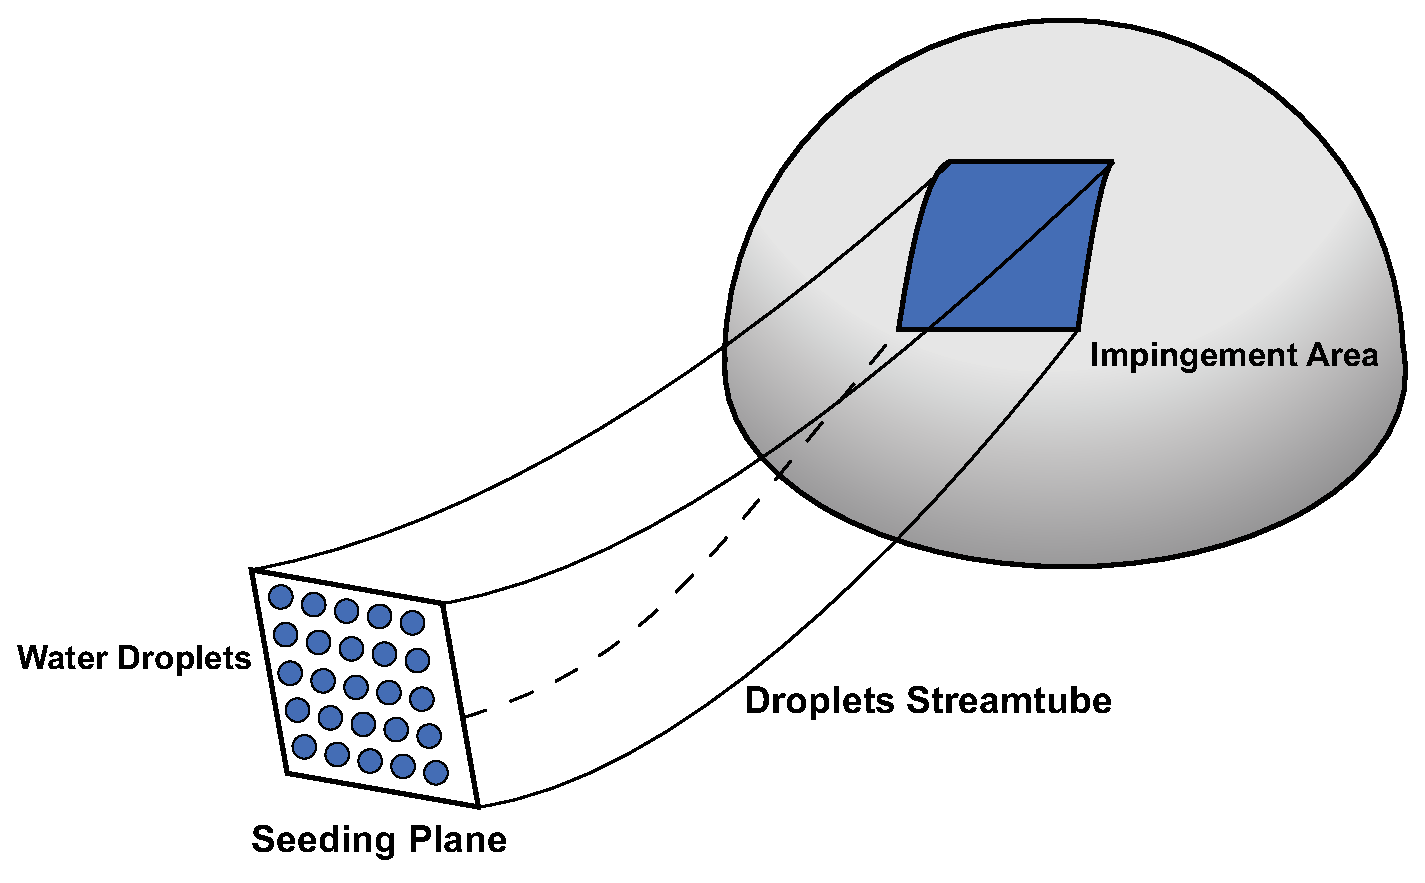
\includegraphics[
    width=\linewidth,
    height=0.43\textheight,
    keepaspectratio
]{FIGURES/LAGRANGIAN/DROP_STREAM_TUBE}

\vspace{0.05cm}
{\small
$\displaystyle\beta = \frac{A_\infty}{A_{\mathrm{imp}}}$
}
\end{column}
\end{columns}

\vspace{0.04cm}
{\color{champsBlue}\bfseries Droplet-Size Distribution}\par
\vspace{0.03cm}
{\small
Either a single \textbf{Mean Volume Diameter (MVD)} or a \textbf{distribution} of bins simulated sequentially and weighted by their fraction of the total LWC.\par}

\vfill
\begin{center}
\begin{tikzpicture}
\node[fill=champsBlue!5, draw=champsBlue!18, rounded corners=4pt,
      text width=0.90\textwidth, inner sep=3pt, align=center, font=\small] {%
  \textbf{Output to thermodynamics:}
  $\dot m_{\mathrm{imp}}$ on the exposed aircraft surface.};
\end{tikzpicture}
\end{center}
\SlideRef{bourgault1999finite,bellosta2023lagrangian}
\end{frame}

\begin{frame}{Air--Droplet Coupling and Droplet Inertia}

\vspace{0.05cm}

\begin{columns}[T,onlytextwidth]

% LEFT COLUMN
\begin{column}{0.48\textwidth}

{\color{champsBlue}\bfseries
One-Way Coupling}

\vspace{0.22cm}

Typical icing conditions:

\[
\mathrm{LWC} \approx 1\ \mathrm{g/m^3},
\qquad
\frac{\mathrm{LWC}}{\rho_w}
\approx 10^{-6}
\]

\vspace{0.12cm}

{\small
The low liquid-water concentration
allows us to neglect droplet feedback
on the airflow.
}

\vspace{0.15cm}

\begin{center}
\begin{tikzpicture}[
    every node/.style={font=\small}
]

\node[
    draw=champsBlue,
    fill=champsBlue!7,
    rounded corners=3pt,
    minimum width=2.4cm,
    minimum height=0.55cm
] (air) at (0,0) {Airflow};

\node[
    draw=champsBlue,
    fill=champsBlue!7,
    rounded corners=3pt,
    minimum width=2.4cm,
    minimum height=0.55cm
] (drop) at (0,-0.95) {Droplets};

\draw[
    ->,
    >=stealth,
    champsBlue,
    very thick
] (air) -- (drop);

\node[
    right,
    font=\scriptsize,
    text=gray
] at (0.1,-0.475) {No feedback};

\end{tikzpicture}
\end{center}

\end{column}

% RIGHT COLUMN
\begin{column}{0.48\textwidth}

{\color{champsBlue}\bfseries
Droplet Inertia: Stokes Number}

\vspace{0.22cm}

\[
St = \frac{\tau_d}{\tau_f}
= \frac{\rho_d D^2 U_\infty}
{18\mu_a c_{\mathrm{ref}}}
\]

\vspace{0.25cm}

{\color{champsBlue}\bfseries
$St \ll 1$}

{\small
Droplets rapidly adapt to changes in
the airflow and closely follow streamlines.
}

\vspace{0.28cm}

{\color{champsBlue}\bfseries
$St \gg 1$}

{\small
Droplet inertia becomes dominant,
leading to greater deviations
from airflow streamlines.
}

\end{column}

\end{columns}

\vfill

\begin{center}
\begin{tikzpicture}
\node[fill=champsBlue!5, draw=champsBlue!18, rounded corners=4pt,
      text width=0.90\textwidth, inner sep=3pt, align=center, font=\small] {%
\textbf{The aerodynamic solution drives
droplet transport, while droplet inertia
governs their response to the flow.}};
\end{tikzpicture}
\end{center}

\SlideRef{clift2005bubbles}
\end{frame}

\begin{frame}{Droplet Impingement: Lagrangian vs. Eulerian}
\vspace{-0.1cm}
\begin{columns}[T,onlytextwidth]
\begin{column}{0.48\textwidth}
\centering
{\color{champsBlue}\bfseries\large Lagrangian}\par
\vspace{0.10cm}
\parbox[c][0.46\textheight][c]{\linewidth}{\centering{\setlength{\fboxsep}{0pt}\setlength{\fboxrule}{0.6pt}\fbox{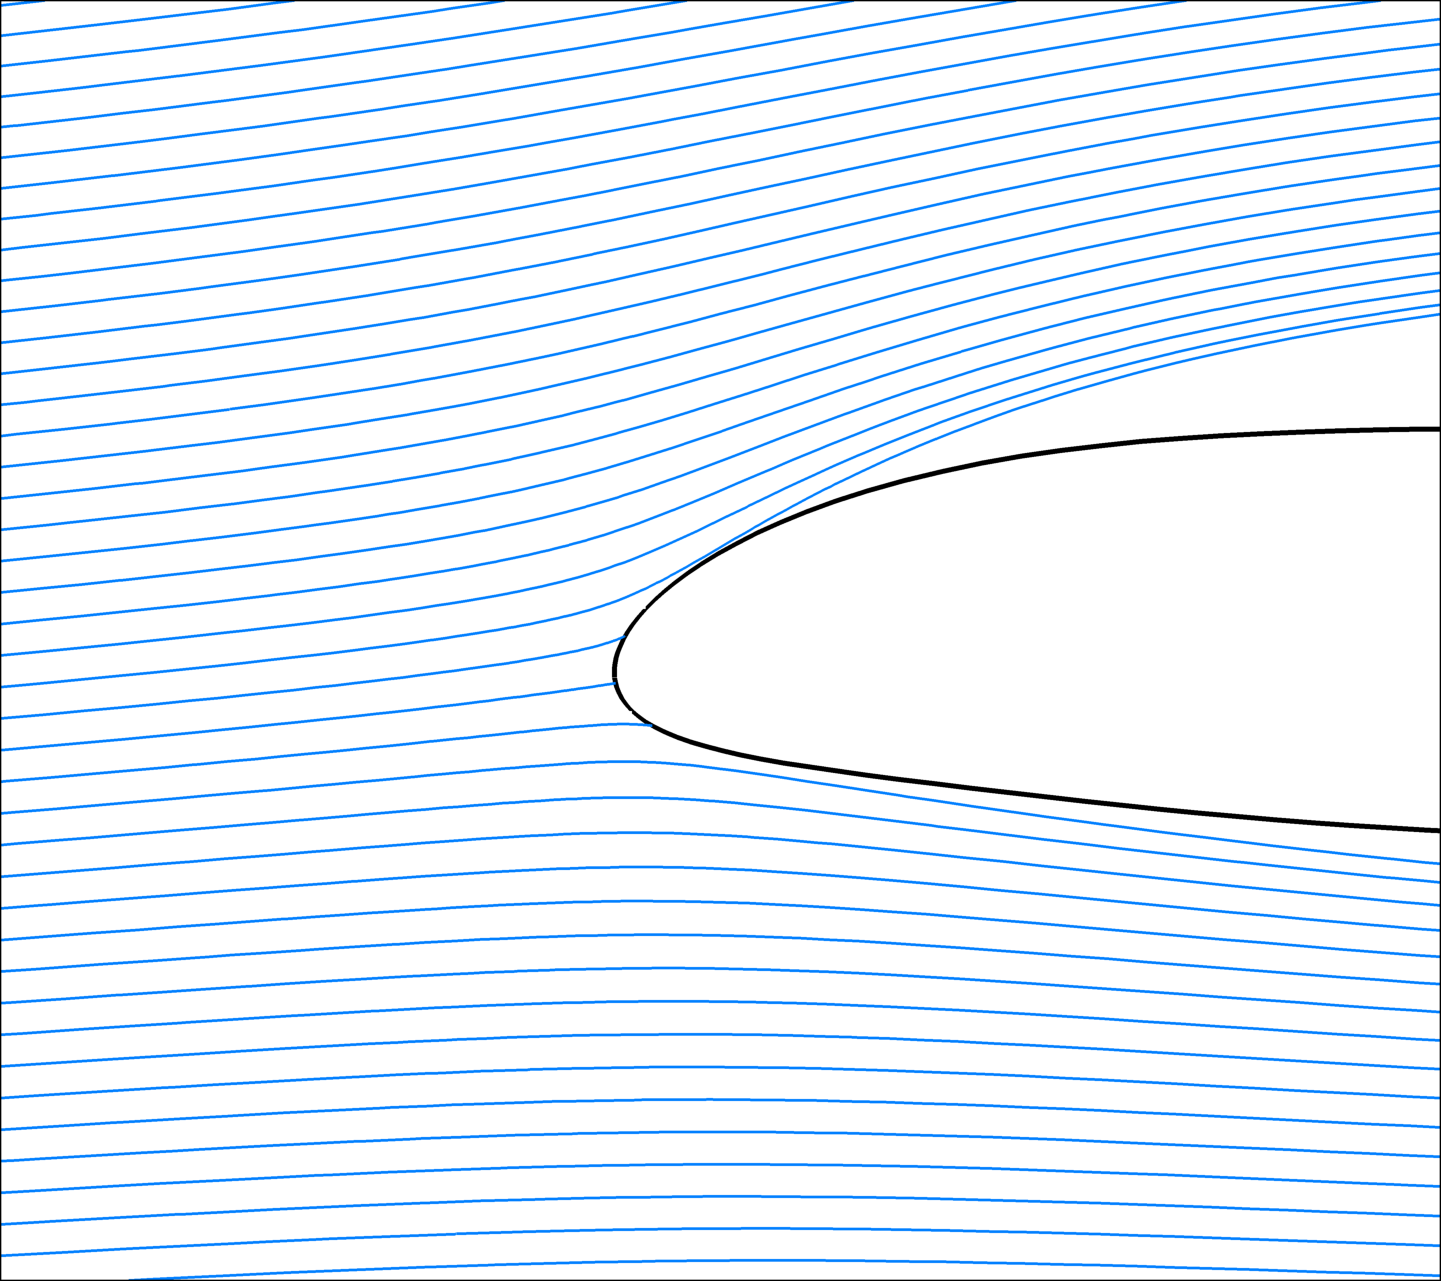
\includegraphics[width=0.96\linewidth,height=0.44\textheight,keepaspectratio]{FIGURES/LAGRANGIAN/DROP_SOLUTION.png}}}}

\vspace{0.10cm}
{\small
\textbf{Particle-based:}
$\mathbf{x}_d(t)$, $\mathbf{u}_d(t)$\par
Individual trajectories integrated through the flow.
\par}
\vspace{0.12cm}
{\scriptsize
{\color{champsBlue}\textbf{ODEs:}}\quad$\left\{\begin{aligned}
\dot{\mathbf{x}}_d&=\mathbf{u}_d\\[-1pt]
\dot{\mathbf{u}}_d&=F(\mathbf{u}_a-\mathbf{u}_d)+\mathbf{g}
\end{aligned}\right.$\par}
\end{column}

\begin{column}{0.48\textwidth}
\centering
{\color{champsBlue}\bfseries\large Eulerian}\par
\vspace{0.10cm}
\parbox[c][0.46\textheight][c]{\linewidth}{\centering{\setlength{\fboxsep}{0pt}\setlength{\fboxrule}{0.6pt}\fbox{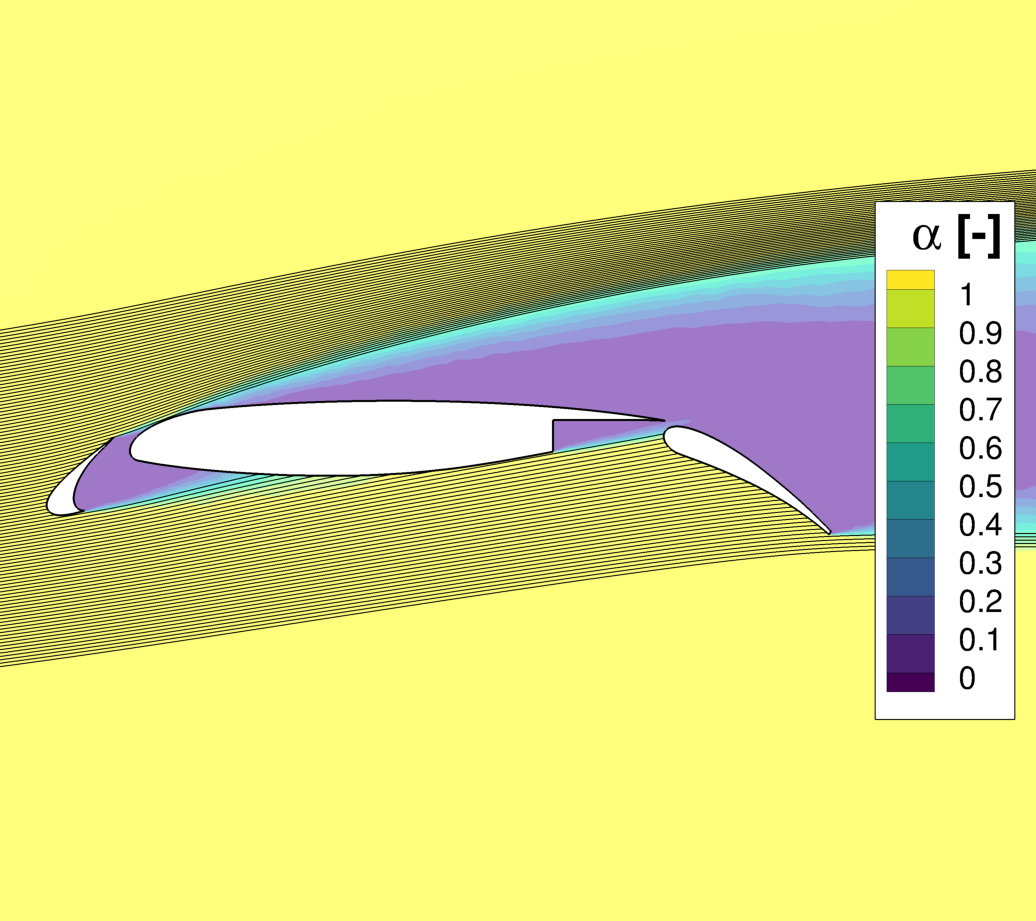
\includegraphics[
    width=0.96\linewidth,
    height=0.44\textheight,
    keepaspectratio
]{FIGURES/LAGRANGIAN/DropletVolumeFraction.png}}}}

\vspace{0.10cm}
{\small
\textbf{Field-based:}
$\alpha(\mathbf{x})$, $\mathbf{u}_d(\mathbf{x})$\par
Continuum equations on the computational mesh.
\par}
\vspace{0.12cm}
{\scriptsize
{\color{champsBlue}\textbf{PDEs:}}\quad$\left\{\begin{aligned}
\partial_t\alpha+\nabla\cdot(\alpha\mathbf{u}_d)&=0\\[-1pt]
\partial_t\mathbf{u}_d+(\mathbf{u}_d\cdot\nabla)\mathbf{u}_d&=F(\mathbf{u}_a-\mathbf{u}_d)+\mathbf{g}
\end{aligned}\right.$\par}
\end{column}
\end{columns}

\vfill
\begin{columns}[T,onlytextwidth]
\begin{column}{0.48\textwidth}
\colorbox{champsBlue!7}{%
\parbox{0.94\linewidth}{\vspace{0.09cm}\centering\scriptsize
\textbf{Advantage:} direct access to impact / SLD physics.\\[1pt]
\textbf{Trade-off:} potentially costly, irregular tracking.
\vspace{0.09cm}}}
\end{column}
\begin{column}{0.48\textwidth}
\colorbox{champsBlue!7}{%
\parbox{0.94\linewidth}{\vspace{0.09cm}\centering\scriptsize
\textbf{Advantage:} regular, scalable field solution.\\[1pt]
\textbf{Trade-off:} numerical dissipation, spurious oscillations.
\vspace{0.09cm}}}
\end{column}
\end{columns}
\SlideRef{bourgault1999finite,bellosta2023lagrangian}
\end{frame}

% ---------------------------------------------------------------------------
% Lagrangian droplet-impingement enhancements (8 slides)
% ---------------------------------------------------------------------------
\providecommand{\LDIhead}[1]{{\color{champsBlue}\bfseries #1}}
\providecommand{\LDIbottom}[1]{%
  \begin{center}%
  \begin{tikzpicture}
  \node[fill=champsBlue!5, draw=champsBlue!18, rounded corners=4pt,
        text width=0.90\textwidth, inner sep=3pt, align=center, font=\small] {#1};
  \end{tikzpicture}%
  \end{center}}

% 1 / 8 --------------------------------------------------------------
\begin{frame}[t]{Adaptive Seeding: Focusing on Impacting Droplets}
\vspace{0.05cm}
Instead of releasing a uniformly dense droplet cloud, concentrate trajectories
where they contribute to surface impingement.
\vspace{0.15cm}
\begin{columns}[T,onlytextwidth]
  \begin{column}{0.485\textwidth}
    \centering
    \LDIhead{Optional: Eulerian-Guided Initialization}\par
    \vspace{0.10cm}
    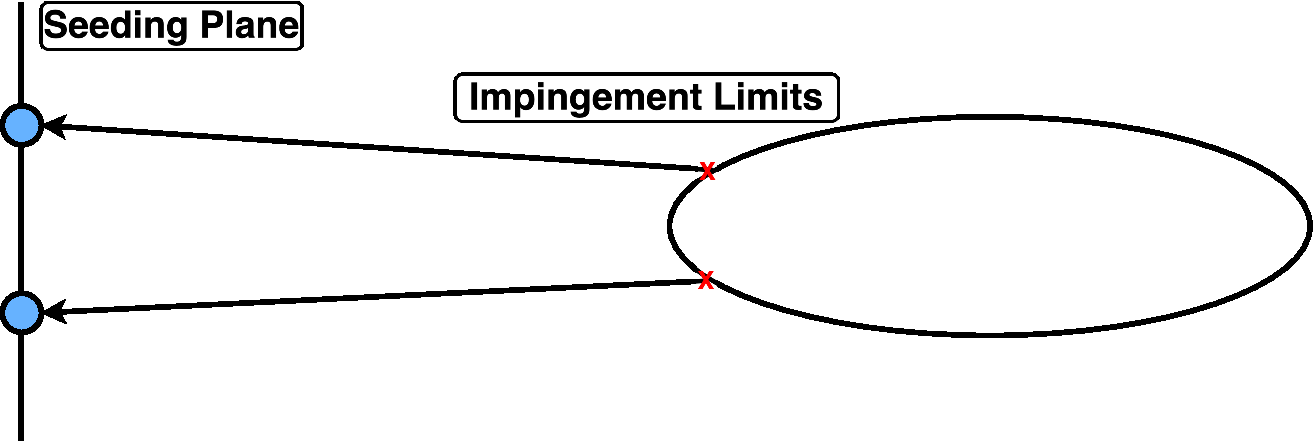
\includegraphics[width=0.97\linewidth,height=2.6cm,keepaspectratio,trim=0 0 210 0,clip]{FIGURES/LAGRANGIAN/seedingPlane-eps-converted-to.pdf}\par
    \vspace{0.02cm}
    {\small Backtrack using Eulerian droplet velocities from the surface to identify the initial upstream seeding region.\par}
  \end{column}
  \begin{column}{0.485\textwidth}
    \centering
    \LDIhead{Main Enhancement: Adaptive Refinement}\par
    \vspace{0.10cm}
    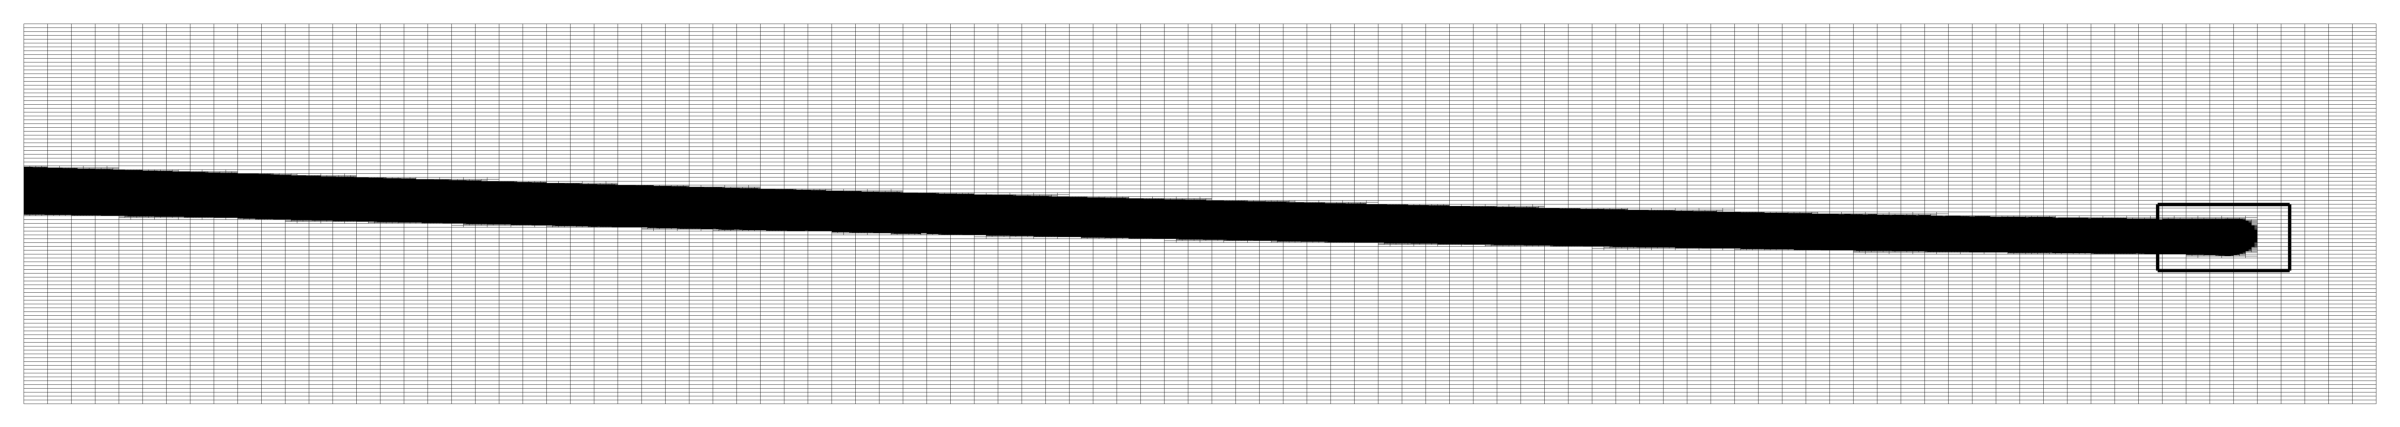
\includegraphics[width=0.97\linewidth]{FIGURES/LAGRANGIAN/seeding_grid_overview.png}\par
    \vspace{0.06cm}
    {\setlength{\fboxsep}{0pt}\setlength{\fboxrule}{0.5pt}\fbox{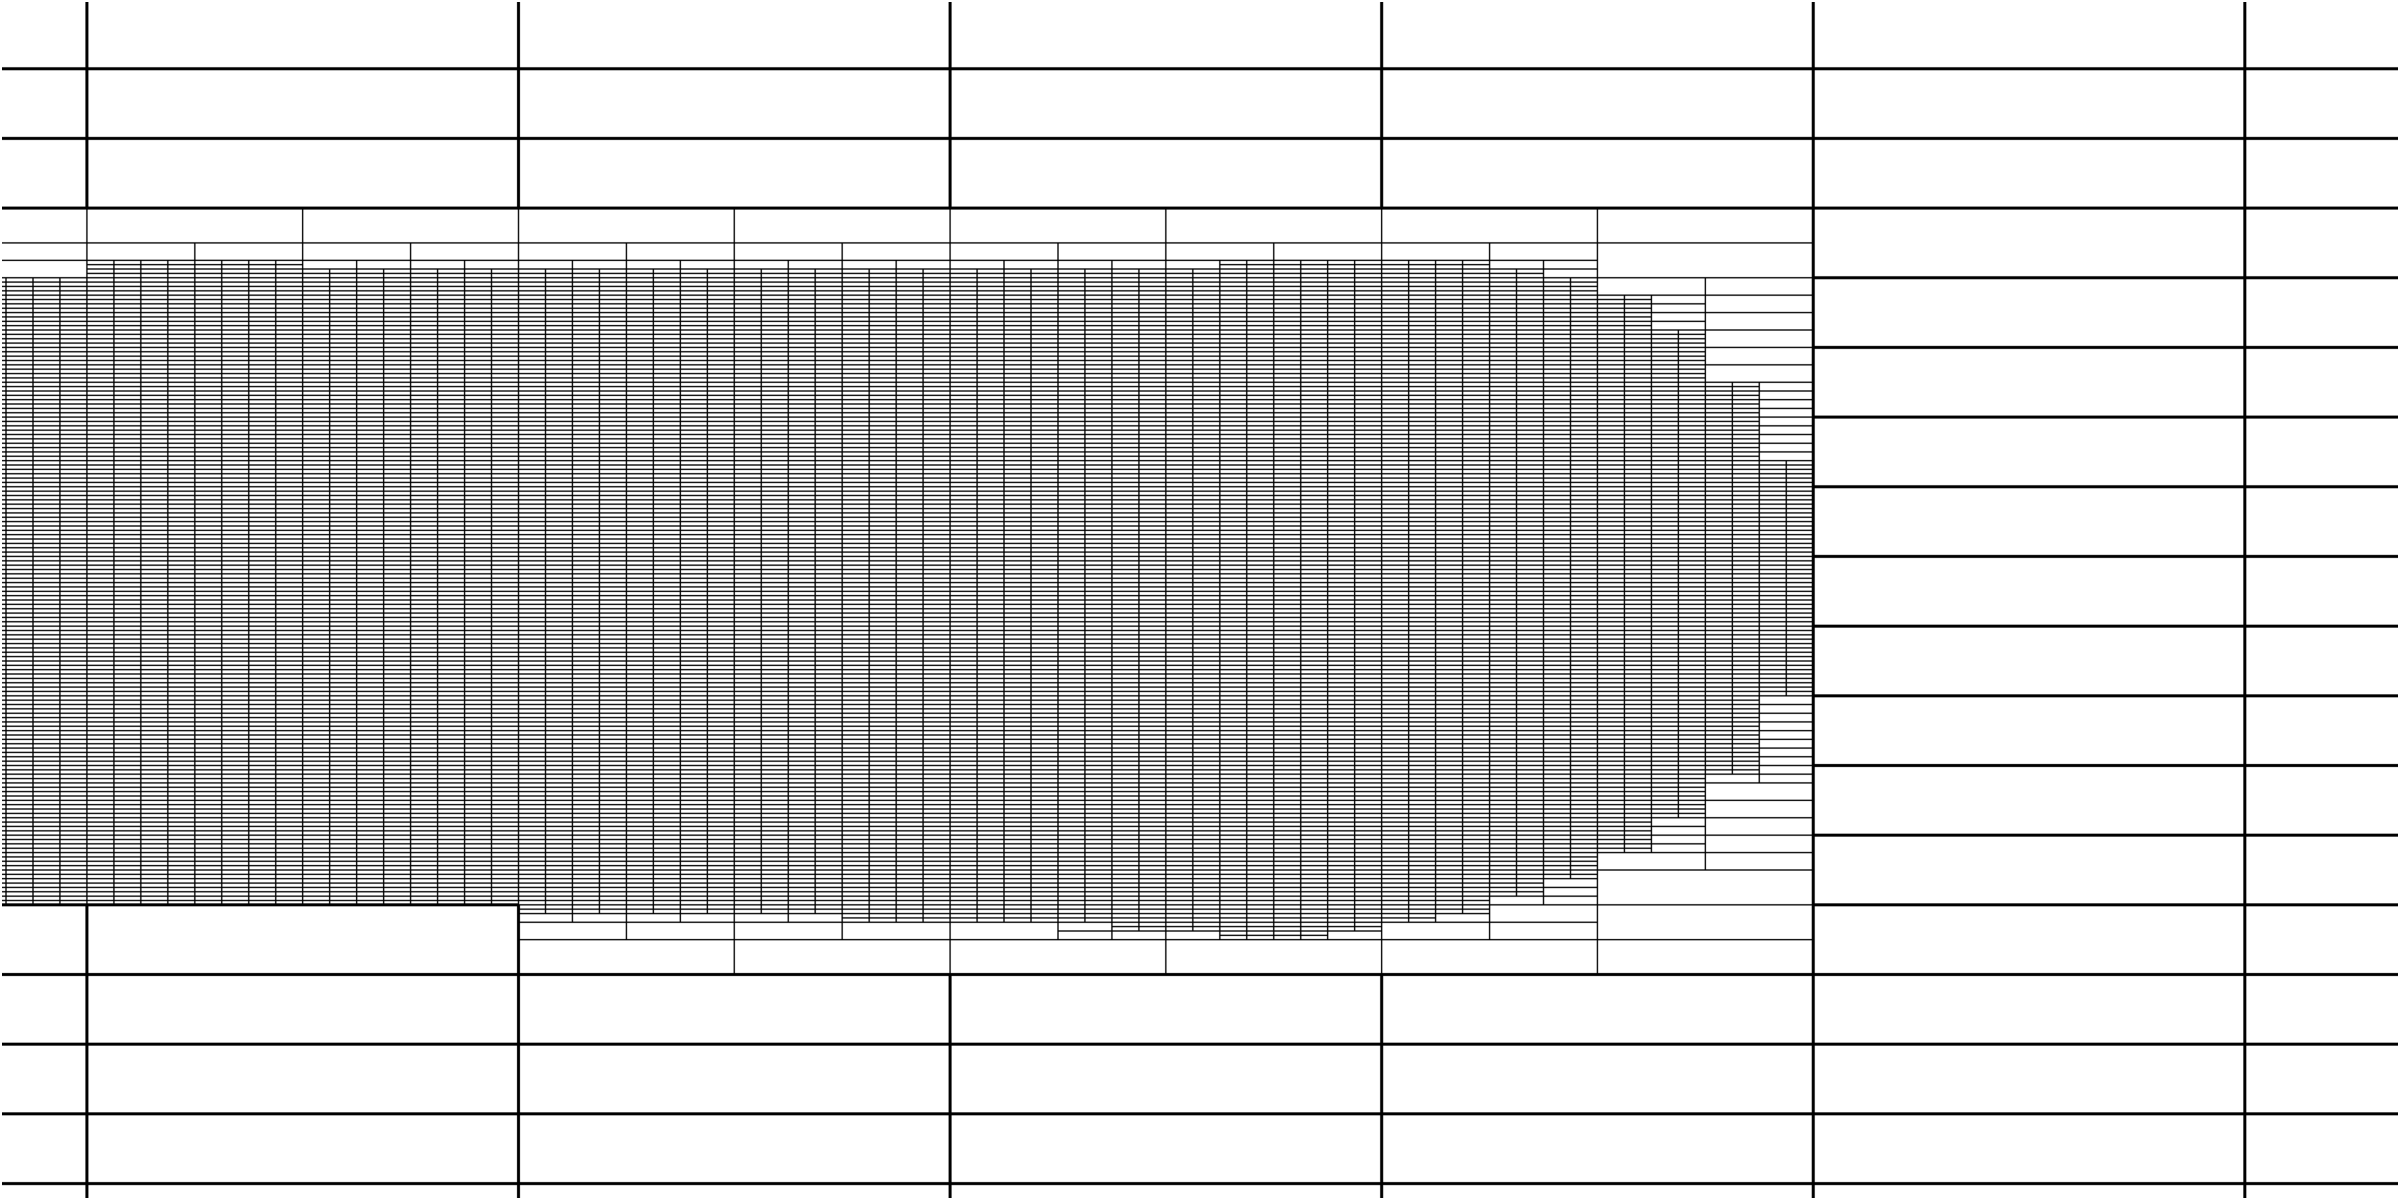
\includegraphics[height=1.55cm]{FIGURES/LAGRANGIAN/seeding_grid_zoom.png}}}\par
    \vspace{0.02cm}
    {\small Refine seeding cells associated with impacting trajectories; reuse previously computed droplets.\par}
  \end{column}
\end{columns}
\vfill
\LDIbottom{\textbf{Goal:} converged collection efficiency with far fewer unnecessary trajectories.\\[2pt]\textbf{Example:} from 10k to 262k seeding nodes (vs.\ 2.5M uniform): \textcolor{green!50!black}{\textbf{$\approx$90\% fewer droplets}}}
\SlideRef{ZAYNI2026112019}
\end{frame}

% 2 / 8 --------------------------------------------------------------
\begin{frame}{Adaptive Seeding: Convergence-Driven Refinement}
\LDIhead{Global Convergence}\par
\vspace{0.15cm}
\begin{itemize}\setlength\itemsep{0.12cm}
  \item Generate and track a coarse initial cloud.
  \item Refine only seeding cells linked to surface impacts.
  \item Monitor change in \textbf{integrated collection efficiency} between refinement passes.
  \item Stop once the prescribed global tolerance is reached.
\end{itemize}
\vspace{0.25cm}
\textbf{Stopping criterion} (successive passes $k-1$, $k$):\par
\vspace{0.25cm}
{\centering
  $\displaystyle\left|\int_S \beta^{(k)}\,dS-\int_S \beta^{(k-1)}\,dS\right| < 10^{-5}$\par}
\vspace{0.3cm}
{\color{champsBlue}Previously computed trajectories are cached and reused.}
\SlideRef{ZAYNI2026112019}
\end{frame}

% 3 / 8 --------------------------------------------------------------
\begin{frame}[t]{Face-to-Face Lagrangian Tracking}
\vspace{0.06cm}
\begin{columns}[c,onlytextwidth]
  \begin{column}{0.46\textwidth}
    \centering
    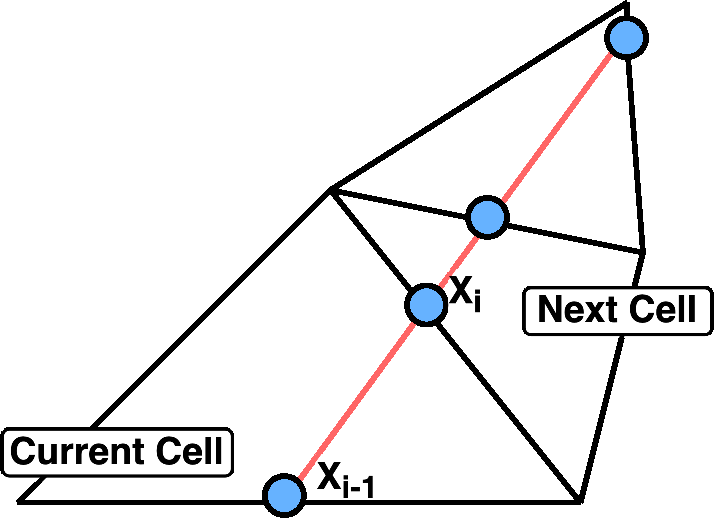
\includegraphics[width=0.99\linewidth,height=3.42cm,keepaspectratio]{FIGURES/LAGRANGIAN/Trackingface2face-eps-converted-to.pdf}\par
    \vspace{0.09cm}
    {\small Successive \textbf{ray--face intersections} identify the next cell through mesh connectivity.\par}
  \end{column}
  \begin{column}{0.51\textwidth}
    \LDIhead{Numerical Integration}\par
    \vspace{0.05cm}
    \begin{itemize}\small\setlength\itemsep{0.08cm}
      \item \textbf{Iterative BDF2} for droplet velocity.
      \item Time step set by the \textbf{local residence time inside the cell}.
      \item Droplet position localization through \textbf{facet intersections}.
      \item Direct identification of surface impact faces.
    \end{itemize}
    \vspace{0.15cm}
    {\centering
    $\boxed{\displaystyle\mathbf{u}_d^n=\frac{F\mathbf{u}_a-b\,\mathbf{u}_d^{n-1}-c\,\mathbf{u}_d^{n-2}+\mathbf{g}}{a+F}}$\par
    \vspace{0.12cm}
    {\scriptsize
    $\begin{aligned}
    a&=\frac{2\Delta t_c+\Delta t_{c-1}}{(\Delta t_c+\Delta t_{c-1})\Delta t_c}, &
    b&=-\frac{\Delta t_c+\Delta t_{c-1}}{\Delta t_c\Delta t_{c-1}},\\[0.1cm]
    c&=\frac{\Delta t_c}{(\Delta t_c+\Delta t_{c-1})\Delta t_{c-1}}, &
    F&=\frac{3C_D\rho_a\left\|\mathbf{u}_a-\mathbf{u}_d\right\|}{4\rho_d D}
    \end{aligned}$\par}
    }
  \end{column}
\end{columns}
\vfill
\SlideRef{ZAYNI2026112019,li2019fast,hairer1996}
\end{frame}

% 4 / 8 --------------------------------------------------------------
\begin{frame}[t]{Ray--Face Intersections: Triangles vs. Quadrilaterals}
\vspace{0.06cm}
\begin{columns}[c,onlytextwidth]
  \begin{column}{0.46\textwidth}
    \centering
    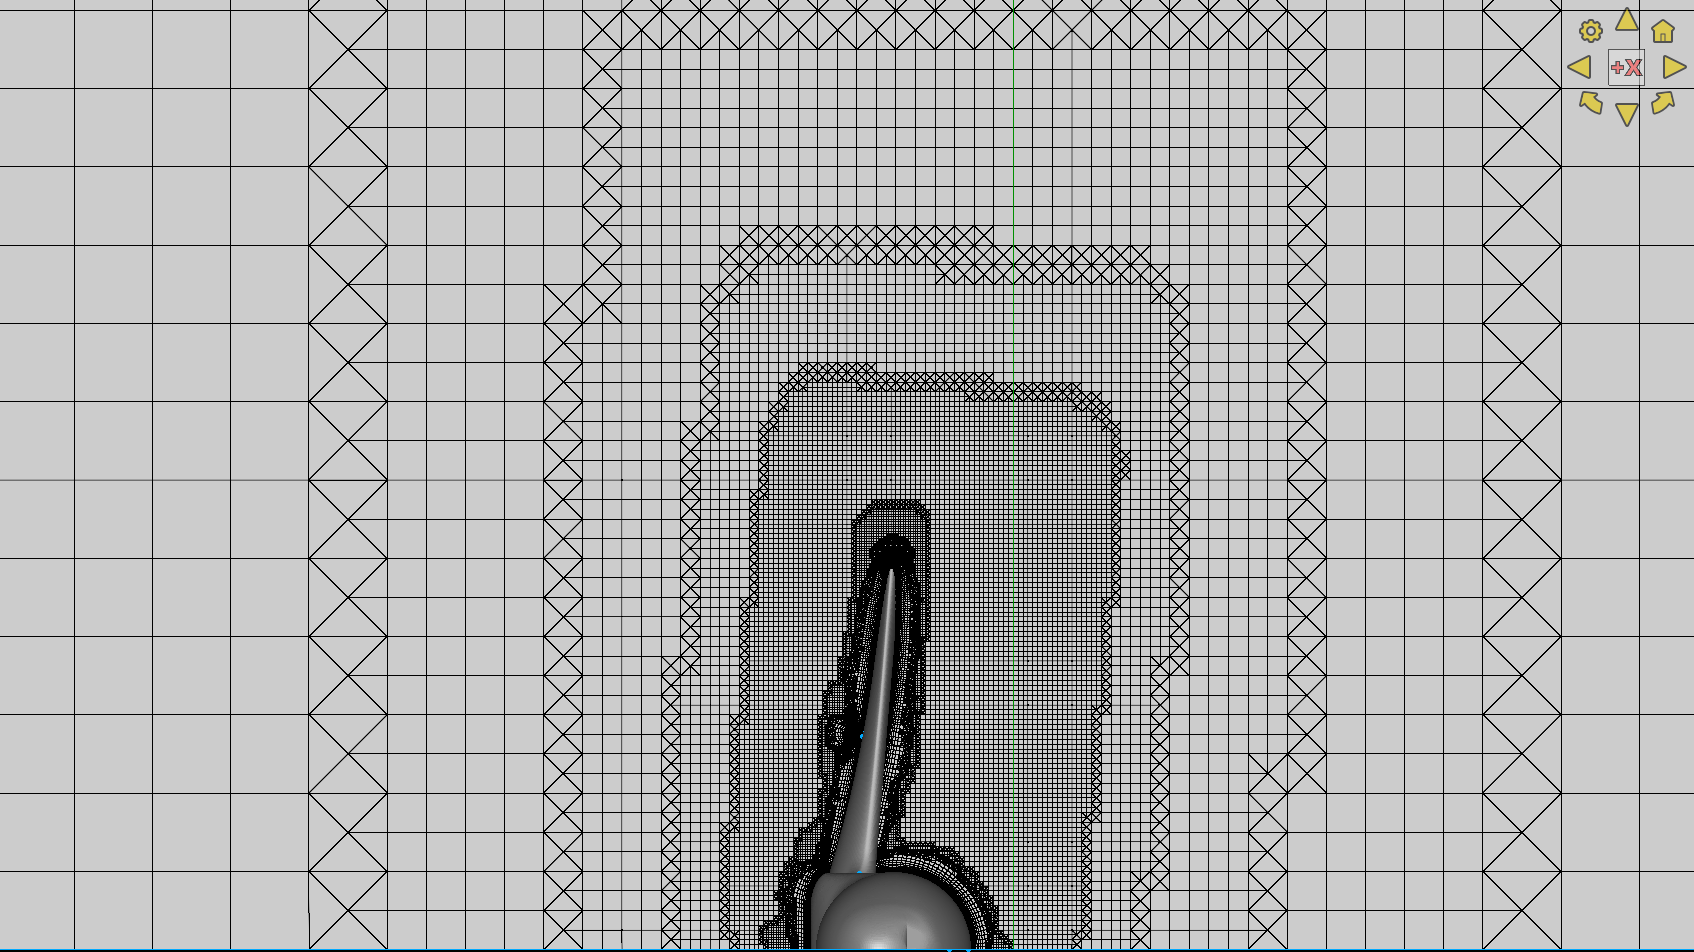
\includegraphics[width=0.99\linewidth,height=3.25cm,keepaspectratio]{FIGURES/LAGRANGIAN/CASE_2p1_MESH_CUT.png}\par
    \vspace{0.10cm}
    {\small Hexahedral-dominant CFD meshes introduce large numbers of quadrilateral faces.\par}
  \end{column}
  \begin{column}{0.51\textwidth}
    \LDIhead{Triangular Faces}\par
    \vspace{0.10cm}
    {\small Planar: standard \textbf{M\"oller--Trumbore} ray--triangle intersection.}\par
    \vspace{0.24cm}
    \LDIhead{Quadrilateral Faces}\par
    \vspace{0.12cm}
    {\small Quad vertices need not be coplanar. Two strategies:}\par
    \begin{enumerate}\setlength\itemsep{0.15cm}
      \item Split into \textbf{two triangles}: simple, but introduces an artificial diagonal.
      \item Treat the face as a \textbf{bilinear patch}: geometry represented continuously.
    \end{enumerate}
    \vspace{0.10cm}
    \[\mathbf p(u,v)=(1-v)\mathbf P_a(u)+v\mathbf P_b(u)\]
    \vspace{-0.08cm}
    {\centering\footnotesize Find \((t,u,v)\) such that \(\mathbf O+t\mathbf D=\mathbf p(u,v)\).\\[1pt]$\Rightarrow$ leads to a \textbf{quadratic equation}, solved by Ramsey et al.\par}
  \end{column}
\end{columns}
\vfill
\LDIbottom{Repeated face intersections make the ray--facet algorithm a computational bottleneck.}
\SlideRef{ZAYNI2026112019}
\end{frame}

% 5 / 8 --------------------------------------------------------------
\begin{frame}[t]{GARP: Fast Ray--Bilinear Patch Intersection}
\vspace{0.06cm}
\begin{columns}[T,onlytextwidth]
  \begin{column}{0.31\textwidth}
    \centering
    \LDIhead{1. Define Geometry}\par\vspace{0.10cm}
    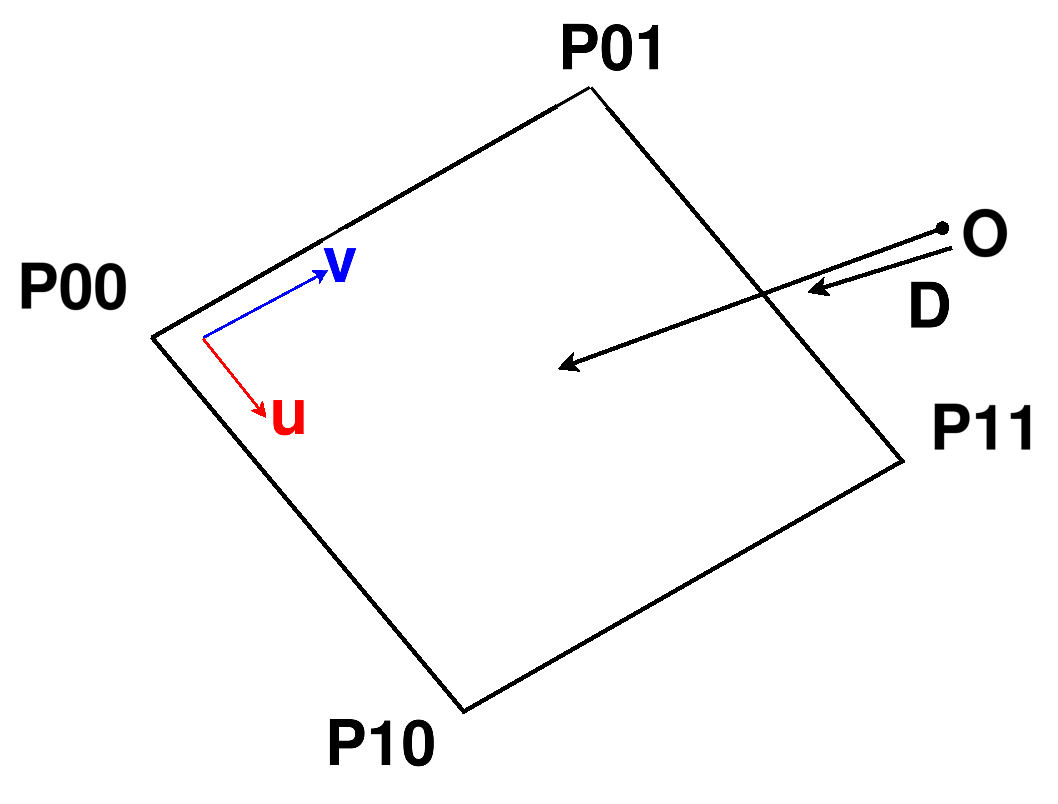
\includegraphics[width=0.98\linewidth,height=2.70cm,keepaspectratio]{FIGURES/LAGRANGIAN/GARP_STEP_0}\par
    {\scriptsize Ray and parametric bilinear patch.\par}
  \end{column}
  \begin{column}{0.31\textwidth}
    \centering
    \LDIhead{2. Determine \(u\)}\par\vspace{0.10cm}
    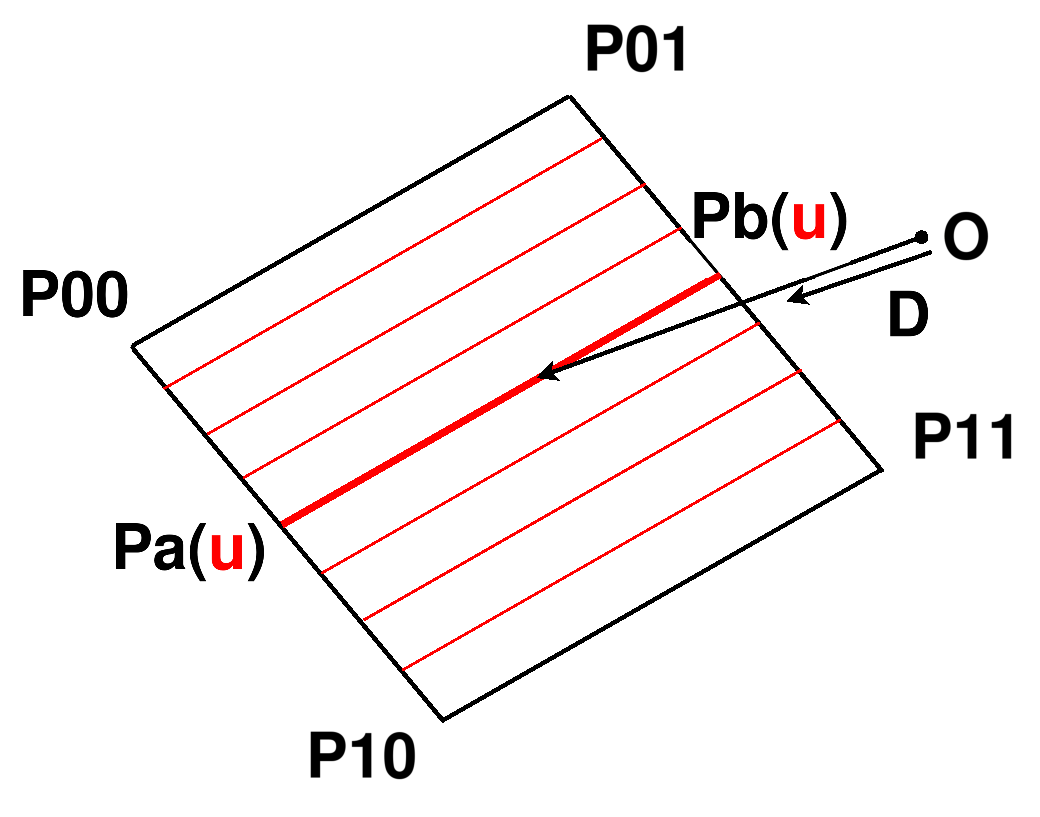
\includegraphics[width=0.98\linewidth,height=2.70cm,keepaspectratio]{FIGURES/LAGRANGIAN/GARP_STEP_1}\par
    {\scriptsize Coplanarity of a ruling segment and ray (quadratic).\par}
  \end{column}
  \begin{column}{0.31\textwidth}
    \centering
    \LDIhead{3. Determine \(v,t\)}\par\vspace{0.10cm}
    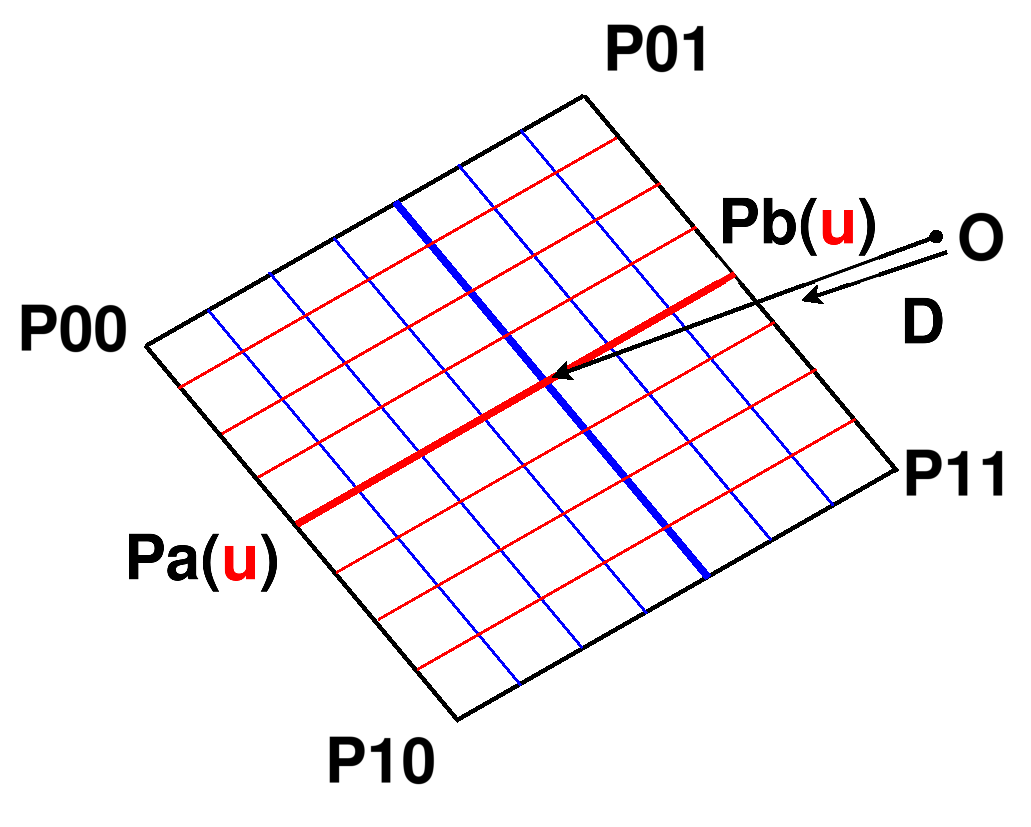
\includegraphics[width=0.98\linewidth,height=2.70cm,keepaspectratio]{FIGURES/LAGRANGIAN/GARP_STEP_2}\par
    {\scriptsize Solve ray--segment geometry; select nearest valid hit.\par}
  \end{column}
\end{columns}
\vspace{0.18cm}
\begin{center}
 {\small\color{champsBlue}\bfseries Execution-Time Reduction (1 million random ray--patch tests)}\par
 \vspace{0.09cm}
 \begin{tabular}{lcc}
  & \textbf{vs. two triangles} & \textbf{vs. Ramsey} \\
  Ramsey bilinear patch & 51.3\% & -- \\
  \rowcolor{green!18}\textbf{GARP bilinear patch} & \textbf{58.2\%} & \textbf{14.2\%} \\
 \end{tabular}
\end{center}
\SlideRef{ZAYNI2026112019}
\end{frame}

% 6 / 8 --------------------------------------------------------------
\begin{frame}[t]{Parallel Lagrangian Tracking: Data Locality and Load Balance}

\vspace{0.08cm}

{\small
Droplets are \textbf{initially distributed} among
the available computational resources.
Essential tracking data are \textbf{replicated across locales}
to minimize inter-node communication.
}

\vspace{0.05cm}

\begin{center}
\begin{tikzpicture}[>=Latex, every node/.style={font=\small}]

% Global aerodynamic solution
\node[
    draw=champsBlue,
    fill=champsBlue!7,
    rounded corners=3pt,
    text width=7.6cm,
    align=center,
    minimum height=0.60cm
] (source) at (0,1.85)
{Distributed Aerodynamic Mesh + Flow Solution};

% Computational locales
\foreach \i/\xx in {1/-3.55,2/0,3/3.55}{

    \node[
        draw=champsBlue!65,
        fill=champsBlue!4,
        rounded corners=3pt,
        align=center,
        text width=2.85cm,
        minimum height=1.65cm
    ] (node\i) at (\xx,-0.15) {
        {\color{champsBlue}\bfseries Locale \i}\\[0.12cm]
        Local flow partition\\
        Other locales' data\\[0.08cm]
        \textbf{Assigned droplets}
    };

    \draw[->,champsBlue!75,thick]
        (source.south) -- (node\i.north);
}

\end{tikzpicture}
\end{center}

\vspace{0.02cm}

\begin{columns}[T,onlytextwidth]
  \begin{column}{0.48\textwidth}
    \LDIhead{Work Distribution}\par
    {\small \textbf{Longest Processing Time (LPT) scheduling}: assign expensive trajectories first; refine runtime estimates between adaptive seeding passes.}\par
  \end{column}
  \begin{column}{0.48\textwidth}
    \LDIhead{Data Locality}\par
    {\small Local access to flow and mesh information avoids remote reads at the cost of \textbf{increased memory usage}.}\par
  \end{column}
\end{columns}

\vfill

\SlideRef{ZAYNI2026112019,parenteau,BALDAN2023105856}

\end{frame}

% Scalability -------------------------------------------------------
\begin{frame}{Lagrangian Solver: Parallel Scalability}

\vspace{-0.05cm}

\begin{columns}[T,onlytextwidth]

% SPEEDUP
\begin{column}{0.49\textwidth}
\centering

{\color{champsBlue}\bfseries Speedup}

\vspace{0.05cm}

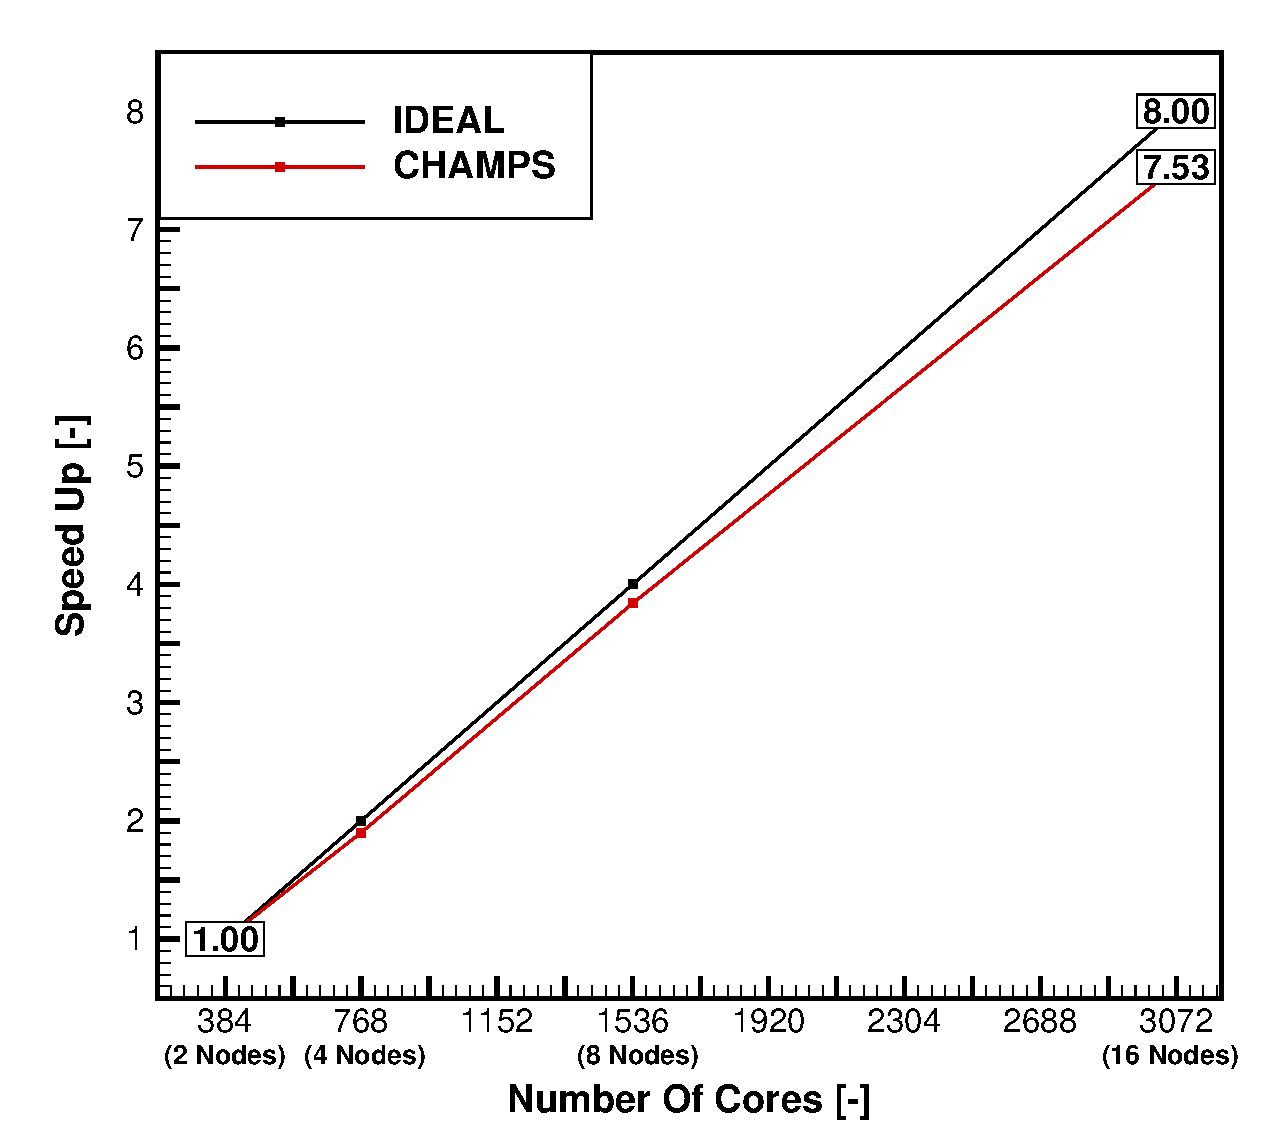
\includegraphics[
    width=\linewidth,
    height=0.56\textheight,
    keepaspectratio
]{FIGURES/LAGRANGIAN/SpeedUp}

\end{column}

% EFFICIENCY
\begin{column}{0.49\textwidth}
\centering

{\color{champsBlue}\bfseries Parallel Efficiency}

\vspace{0.05cm}

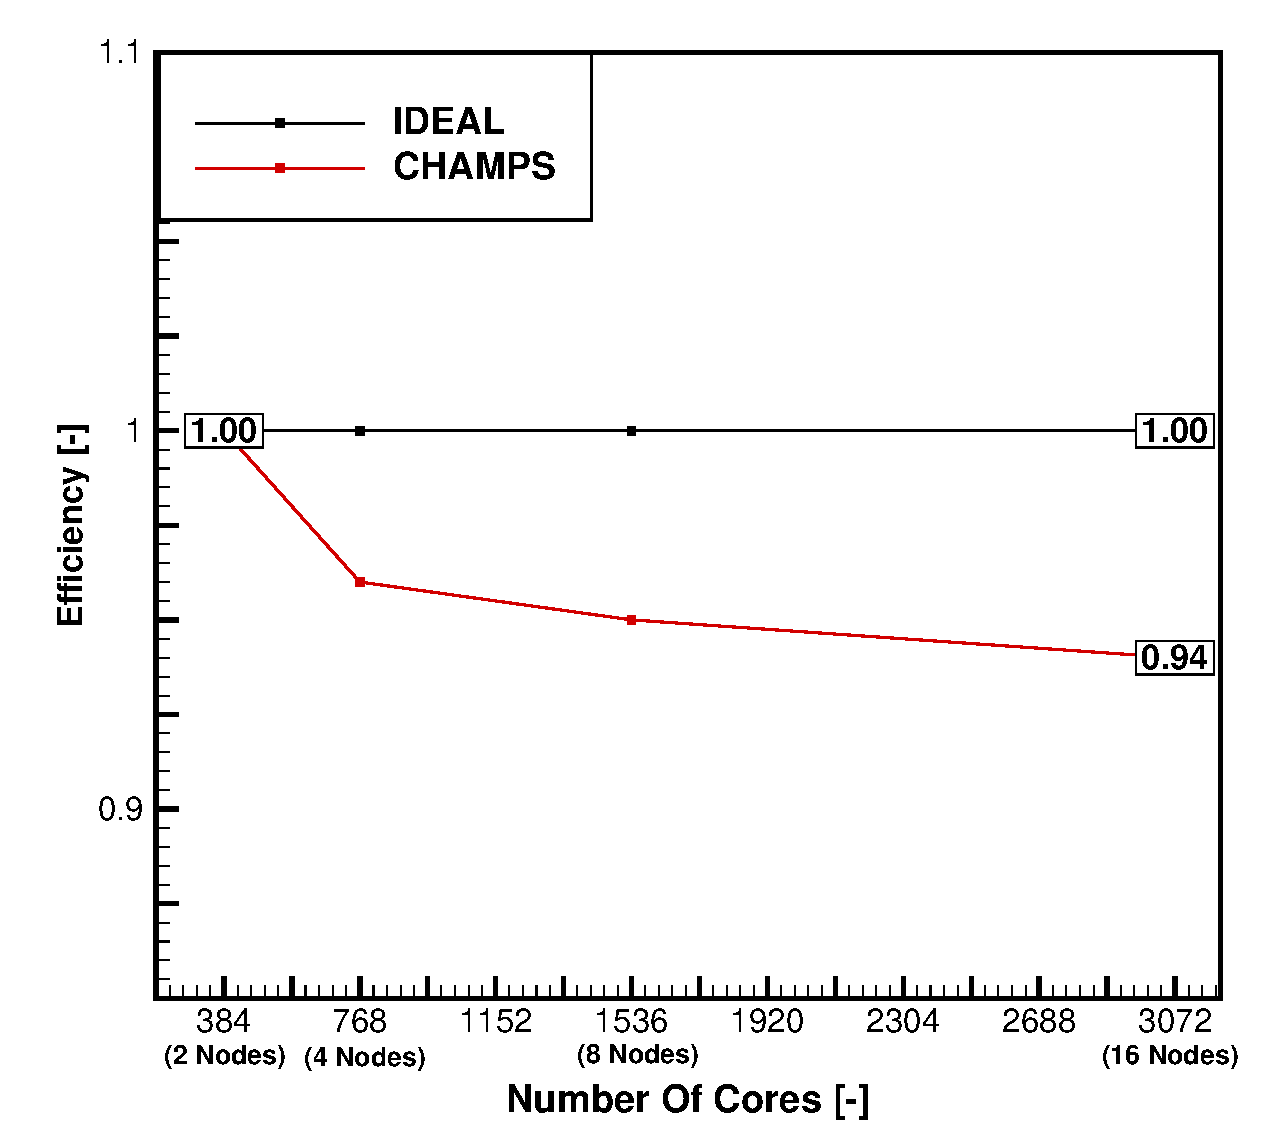
\includegraphics[
    width=\linewidth,
    height=0.56\textheight,
    keepaspectratio
]{FIGURES/LAGRANGIAN/Efficiency}

\end{column}

\end{columns}

\vspace{0.05cm}

\begin{center}
{\scriptsize
\textbf{Benchmark:} IPW2 Case 1.3
\quad $\vert$ \quad
12.8 million droplets
\quad $\vert$ \quad
384--3072 cores (2--16 nodes)\\[1pt]
\textbf{Trillium:} 2 $\times$ AMD EPYC 9655 per node (192 cores/node)
}
\end{center}

\vspace{-0.1cm}

\begin{center}
\begin{tikzpicture}
\node[fill=champsBlue!5, draw=champsBlue!18, rounded corners=4pt,
      text width=0.92\textwidth, inner sep=3pt, align=center, font=\small] {%
\textbf{\color{champsBlue}$7.53\times$ speedup and $94\%$ efficiency at 3072 cores (16 nodes).}\\[1pt]
Good strong-scaling performance on distributed-memory HPC systems.};
\end{tikzpicture}
\end{center}

\SlideRef{ZAYNI2026112019}
\end{frame}

% 7 / 8 --------------------------------------------------------------
\begin{frame}[t]{Supercooled Large Droplets: Pre-Impact and Impact Physics}
\vspace{0.04cm}
\begin{columns}[T,onlytextwidth]
  \begin{column}{0.48\textwidth}
    \centering
    \LDIhead{Pre-Impact: Deformation}\par
    \vspace{0.08cm}
    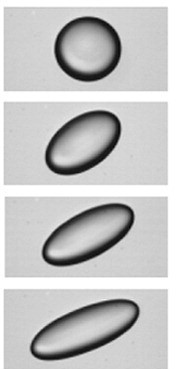
\includegraphics[width=\linewidth,height=3.9cm,keepaspectratio]{FIGURES/LAGRANGIAN/DROPLET_DEFORMATION.jpg}\par
    \vspace{0.08cm}
    {\small\textbf{Second-order effect:} changes effective drag, hence velocity and trajectory.\par}
    \vspace{0.12cm}
    \tikz\node[fill=champsBlue!7, rounded corners=4pt, inner xsep=0.3cm, inner ysep=0.12cm, font=\small]{$C_D=(1-f)C_{D,\mathrm{sphere}}+fC_{D,\mathrm{disk}}$};\par
  \end{column}
  \begin{column}{0.48\textwidth}
    \centering
    \LDIhead{At Impact: Splashing}\par
    \vspace{0.08cm}
    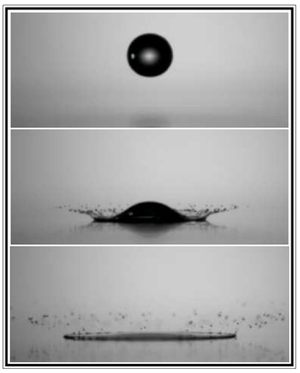
\includegraphics[width=\linewidth,height=3.9cm,keepaspectratio]{FIGURES/LAGRANGIAN/DROPLET_SPLASHING.png}\par
    \vspace{0.08cm}
    {\small\textbf{First-order effect:} a semi-empirical impact model predicts how much water is retained.\par}
    \vspace{0.12cm}
    \tikz\node[fill=champsBlue!7, rounded corners=4pt, inner xsep=0.3cm, inner ysep=0.12cm, font=\small]{$\beta_{\mathrm{retained}}=(1-f_m)\beta_0$};\par
  \end{column}
\end{columns}
\vfill
\SlideRef{wright2004semi,trontin2016revisited,honsek2006fensap}
\end{frame}

% ---------------------------------------------------------
% SLD splashing models: Wright vs ONERA
% ---------------------------------------------------------
\begin{frame}{SLD Modeling: Wright vs. ONERA}

\vspace{-0.1cm}

{\small
Semi-empirical models account for droplet splashing
and the fraction of water retained after impact.
}

\vspace{0.1cm}

\begin{columns}[T,onlytextwidth]

% WRIGHT
\begin{column}{0.48\textwidth}

{\color{champsBlue}\bfseries
Wright et al.}

\vspace{0.08cm}

{\small Mass-loss coefficient:}

{\small\vspace{-0.25cm}
\[
\begin{aligned}
f_m &= 0.7(1-\sin\theta_0)\\
&\quad\times
\left[1-\exp\left(-0.0092(K_M-200)\right)\right]
\end{aligned}
\]}

\vspace{-0.12cm}

{\scriptsize
Splashing criterion: $K_M>200$,
$\theta_0<\pi/2$, with\par\vspace{0.03cm}
{\centering$K_M=\dfrac{0.859\,K^{1/2}\left(\rho_w/\mathrm{LWC}\right)^{1/8}}{\sin^{5/4}(\theta_0)}$,\quad $K=Oh\,Re_d^{5/4}$\par}
}

\end{column}

% ONERA / TRONTIN
\begin{column}{0.48\textwidth}

{\color{champsBlue}\bfseries
ONERA -- Trontin et al.}

\vspace{0.08cm}

{\small Mass-loss coefficient:}

{\small\vspace{-0.25cm}
\[
f_m =
1-
g\left(\frac{\theta}{\theta_c}\right)
f\left(\frac{K_c-K_0}{K_0}\right)
\]}

\vspace{0.05cm}

{\scriptsize
Splashing criterion:
$K_c=We\,Oh^{-2/5}>K_0=657$.
}

\end{column}

\end{columns}

\vspace{0.08cm}

\hrule

\vspace{0.08cm}

{\color{champsBlue}\bfseries
Wright: Secondary-Droplet Reinjection}

\vspace{0.04cm}
{\centering\small
$u_{n,\mathrm{post}}=u_{n,\mathrm{imp}}\left(1.075-0.0025\,\alpha_{\mathrm{imp}}\right),\qquad
u_{t,\mathrm{post}}=u_{t,\mathrm{imp}}\left(0.300-0.0020\,\alpha_{\mathrm{imp}}\right),$\\[0.08cm]
$D_{\mathrm{new}}=D\,\exp(-0.0281K_M)$\par}

\vspace{0.04cm}

{\scriptsize
The ejected mass is represented by a secondary-droplet
parcel, tracked until domain exit or reimpingement.
}

\vfill

\LDIbottom{\textbf{Collection-efficiency correction:}
\mbox{$\beta_{\mathrm{retained}}=(1-f_m)\,\beta_0$}\\(Wright: secondary reimpingement can also be added).}
\begin{tikzpicture}[remember picture,overlay]
  \node[anchor=south west,font=\tiny,text=gray,inner sep=0pt]
      at ([xshift=0.1cm,yshift=0.27cm]current page.south west)
      {\cite{wright2004semi,trontin2016revisited}\qquad $We=\frac{\rho_w U_d^2 D}{\sigma_w},\quad Oh=\frac{\mu_w}{\sqrt{\rho_w\sigma_w D}}$};
\end{tikzpicture}
\end{frame}


% 8 / 8 --------------------------------------------------------------
\begin{frame}[t]{SLD: Secondary-Droplet Reimpingement}
\vspace{0.04cm}
\begin{columns}[c,onlytextwidth]
  \begin{column}{0.57\textwidth}
    \centering
    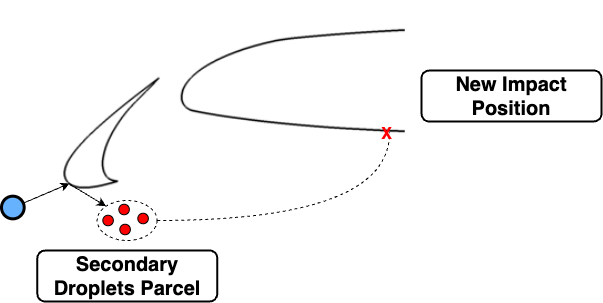
\includegraphics[width=0.99\linewidth,height=3.60cm,keepaspectratio]{FIGURES/LAGRANGIAN/dropletSplashing.png}\par
    \vspace{0.07cm}
    {\small Secondary parcels are launched from a splash event and tracked toward possible downstream impacts.\par}
  \end{column}
  \begin{column}{0.40\textwidth}
    \LDIhead{Wright-Type Splashing Model}\par
    \vspace{0.12cm}
    \begin{enumerate}\setlength\itemsep{0.16cm}
      \item Evaluate impact velocity and angle.
      \item Estimate splashed mass fraction.
      \item Inject secondary-droplet parcels.
      \item Track new trajectories and impacts.
    \end{enumerate}
  \end{column}
\end{columns}
\vfill
\begin{center}
\begin{tikzpicture}
\node[fill=champsBlue!7, rounded corners=4pt, inner xsep=0.4cm, inner ysep=0.05cm]{%
$\begin{aligned}
\beta_{\mathrm{reimp}}&=\frac{m_{\mathrm{sd}}(\mathbf{u}_{\mathrm{sd}}\cdot\mathbf{n})/A_s}{m_\infty U_\infty/A_\infty}\\[0.15cm]
\beta_{\mathrm{final}}&=(1-f_m)\beta_0+\sum_{\mathrm{reimp}}\beta_{\mathrm{reimp}}
\end{aligned}$};
\end{tikzpicture}
\end{center}
\vfill
\SlideRef{wright2004semi,trontin2016revisited}
\end{frame}

% ---------------------------------------------------------------------------
% LDI results (3 slides)
% ---------------------------------------------------------------------------
% #1: geometric description, #2: Mach, #3: alpha, #4: T_inf,
% #5: Re, #6: MVD, #7: c_ref
\providecommand{\LDIResultCaseHeader}[8][]{%
\if\relax\detokenize{#1}\relax
\begin{columns}[T,onlytextwidth]
  \begin{column}{0.30\textwidth}
    {\color{champsBlue}\bfseries\scriptsize GEOMETRY}\vspace{0.05cm}
    \fcolorbox{champsBlue!24}{champsBlue!3}{%
      \parbox[c][1.17cm][c]{0.94\linewidth}{%
        \centering\scriptsize\color{champsBlue!70!black}
        Geometry figure\\[0.04cm]
        \textbf{#2}
      }%
    }
  \end{column}
  \begin{column}{0.67\textwidth}
    {\color{champsBlue}\bfseries\scriptsize CASE PARAMETERS}\par
    \vspace{0.12cm}
    {\centering\small\color{champsBlue}\bfseries
    $\bm{M_\infty=#3}$ \quad \textbf{AoA} $\bm{=#4^\circ}$ \if\relax\detokenize{#5}\relax\else\quad $T_\infty=#5$ K\fi\\[0.1cm]
    $\bm{Re=#6}$ \quad MVD $=#7\,\mu$m \quad $\bm{c_\mathrm{ref}=#8}$ m\par}
  \end{column}
\end{columns}
\else
\begin{columns}[T,onlytextwidth]
  \begin{column}{0.40\textwidth}
    {\color{champsBlue}\bfseries\scriptsize GEOMETRY}\vspace{0.05cm}
    \fcolorbox{champsBlue!24}{champsBlue!3}{%
      \parbox[c][1.0cm][c]{0.96\linewidth}{%
        \centering\scriptsize\color{champsBlue!70!black}
        \includegraphics[width=\linewidth,height=0.62cm,keepaspectratio]{#1}\\[0.04cm]
        \textbf{#2}
      }%
    }
  \end{column}
  \begin{column}{0.57\textwidth}
    {\color{champsBlue}\bfseries\scriptsize CASE PARAMETERS}\par
    \vspace{0.12cm}
    {\centering\small\color{champsBlue}\bfseries
    $\bm{M_\infty=#3}$ \quad \textbf{AoA} $\bm{=#4^\circ}$\\[0.1cm]
    $\bm{Re=#6}$ \quad MVD $=#7\,\mu$m \quad $\bm{c_\mathrm{ref}=#8}$ m\if\relax\detokenize{#5}\relax\else\quad $T_\infty=#5$ K\fi\par}
  \end{column}
\end{columns}
\fi
\vspace{0.05cm}
\endgraf
{\color{champsBlue!20}\rule{\textwidth}{0.5pt}}
\vspace{-0.1cm}
}

\providecommand{\HtailSide}{%
  {\color{champsBlue}\bfseries\scriptsize GEOMETRY}\par\vspace{0.05cm}
  \fcolorbox{champsBlue!24}{champsBlue!3}{%
    \parbox[c][1.25cm][c]{0.94\linewidth}{\centering\scriptsize\color{champsBlue!70!black}
      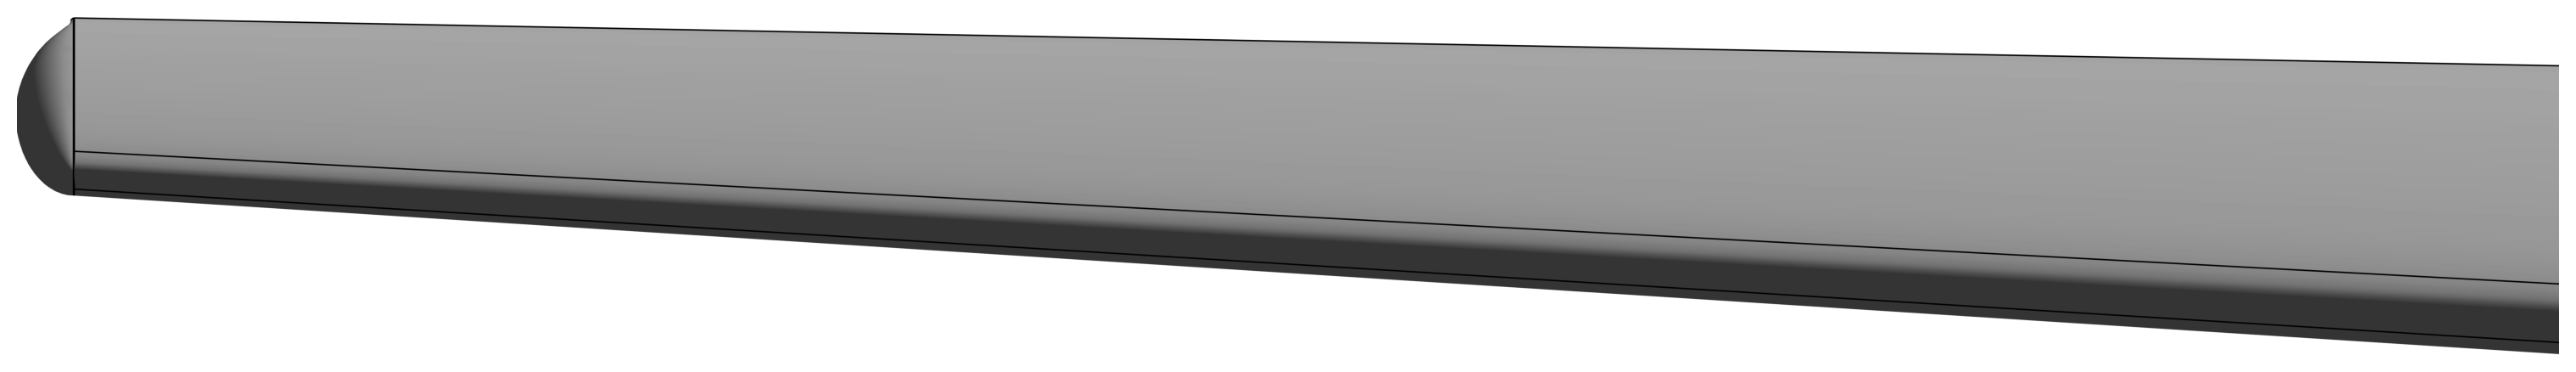
\includegraphics[width=\linewidth,height=0.85cm,keepaspectratio]{FIGURES/LAGRANGIAN/HTAIL_HORIZONTAL.png}\\[0.04cm]
      \textbf{NACA 64A008 H-tail}}}\par
  \vspace{0.3cm}
  {\color{champsBlue}\bfseries\scriptsize CASE PARAMETERS}\par\vspace{0.1cm}
  {\centering\small\color{champsBlue}\bfseries
  $\bm{M_\infty=0.23}$ \quad \textbf{AoA} $\bm{=6^\circ}$\\[0.1cm]
  $\bm{Re=5.0\times10^6}$\\[0.1cm]
  MVD $=92\,\mu$m \quad $\bm{c_\mathrm{ref}=0.956}$ m\par}}

\begin{frame}{IPW1-112: Eulerian vs. Lagrangian Results}
\begin{columns}[c,onlytextwidth]
  \begin{column}{0.33\textwidth}
    \HtailSide
  \end{column}
  \begin{column}{0.66\textwidth}\centering
    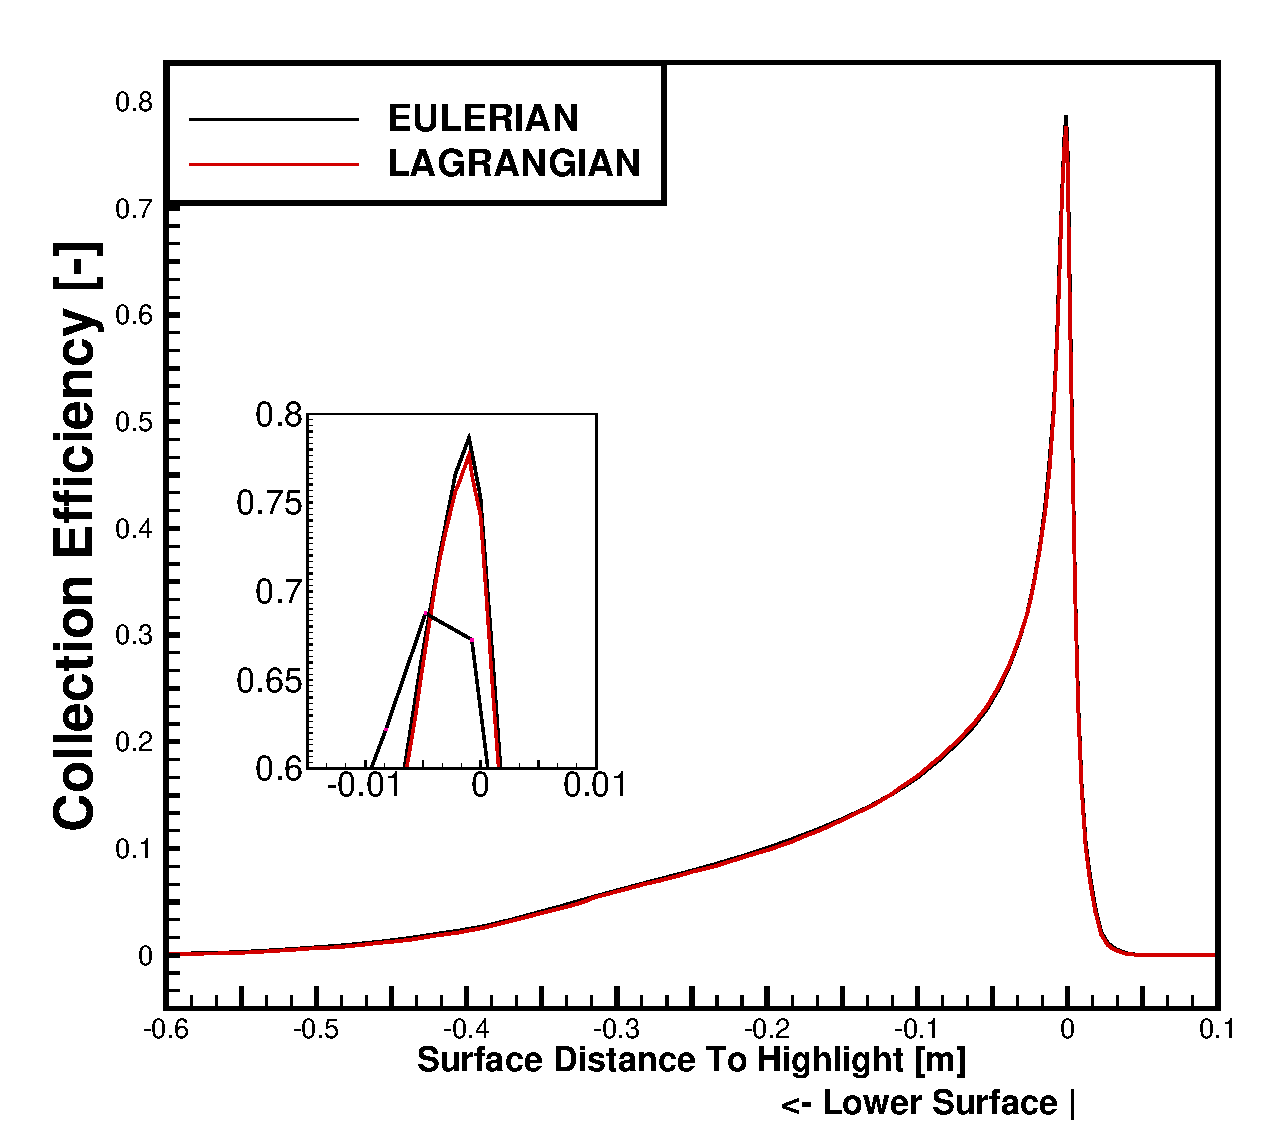
\includegraphics[width=\linewidth,height=6.3cm,keepaspectratio]{FIGURES/LAGRANGIAN/CASE_112_DISTRIBUTION}
  \end{column}
\end{columns}
\vfill
\begin{center}
\begin{tikzpicture}
\node[fill=champsBlue!5, draw=champsBlue!18, rounded corners=4pt,
      text width=0.92\textwidth, inner sep=3pt, align=center, font=\small] {%
Excellent Eulerian--Lagrangian agreement, but not yet with experiments.};
\end{tikzpicture}
\end{center}
\SlideRef{laurendeau2022summary,papadakis2007large}
\end{frame}

\begin{frame}{IPW1-112: Effect of SLD Models}
\begin{columns}[c,onlytextwidth]
  \begin{column}{0.33\textwidth}
    \HtailSide
  \end{column}
  \begin{column}{0.66\textwidth}\centering
    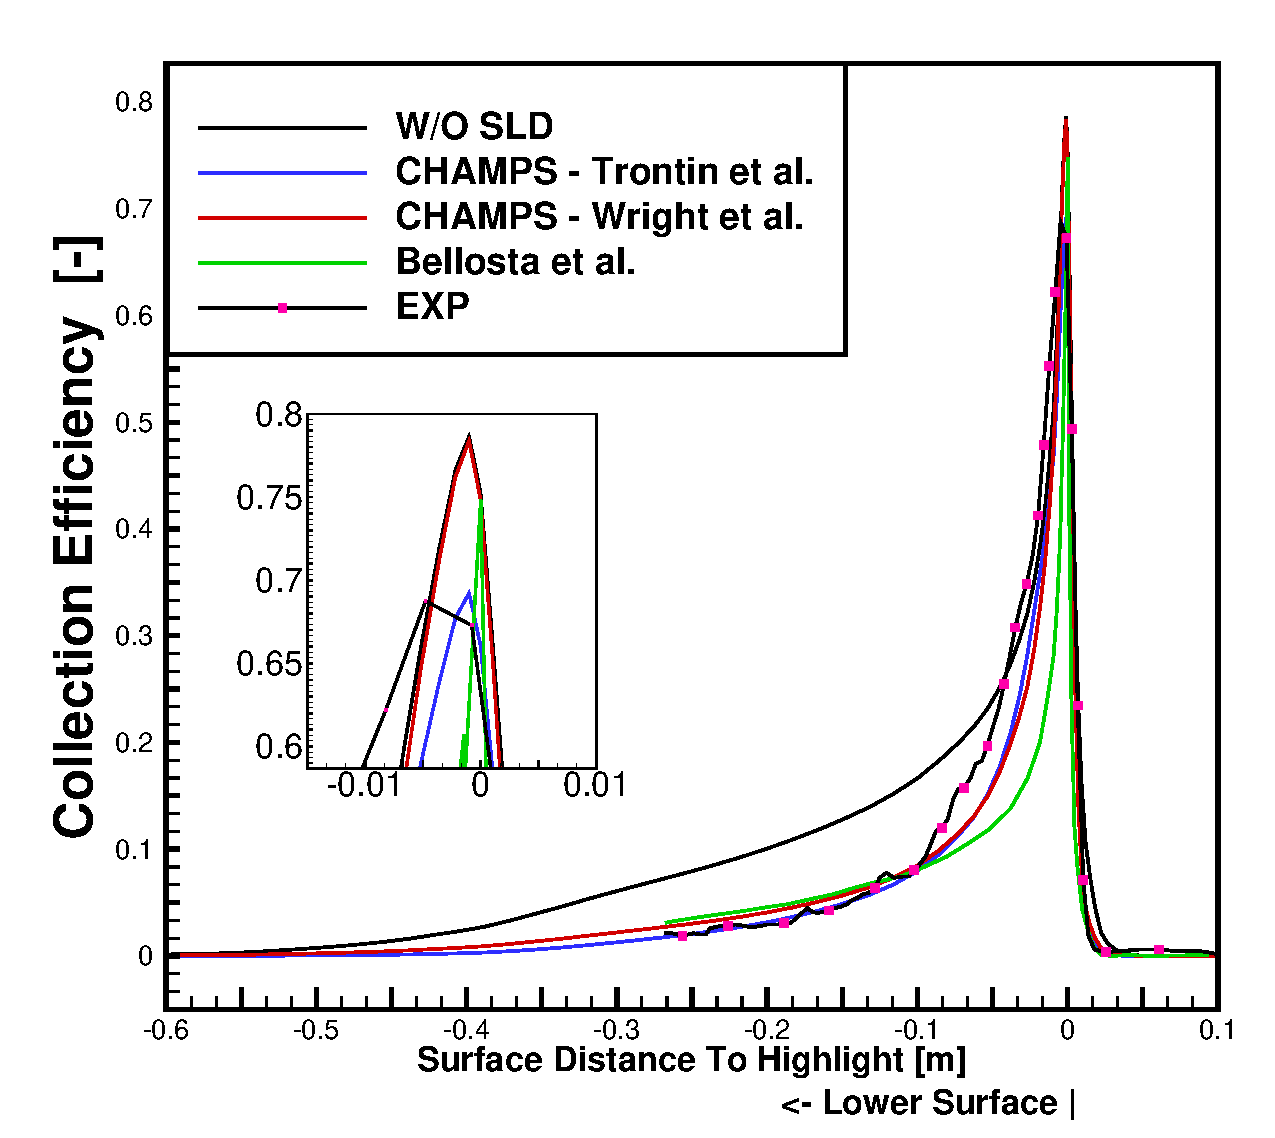
\includegraphics[width=\linewidth,height=6.3cm,keepaspectratio]{FIGURES/LAGRANGIAN/CASE_112_SLD}
  \end{column}
\end{columns}
\vfill
\begin{center}
\begin{tikzpicture}
\node[fill=champsBlue!5, draw=champsBlue!18, rounded corners=4pt,
      text width=0.92\textwidth, inner sep=3pt, align=center, font=\small] {%
SLD corrections improve agreement.};
\end{tikzpicture}
\end{center}
\SlideRef{laurendeau2022summary,papadakis2007large}
\end{frame}

\begin{frame}{IPW1-122: SLD Impingement on a Multi-Element Airfoil}
\LDIResultCaseHeader[FIGURES/LAGRANGIAN/MDA_GEOMETRY.png]{Slat / main / flap}{0.23}{4}{}{4.8\times 10^6}{92}{0.914}
\begin{columns}[T,onlytextwidth]
  \begin{column}{0.29\textwidth}
    \centering
    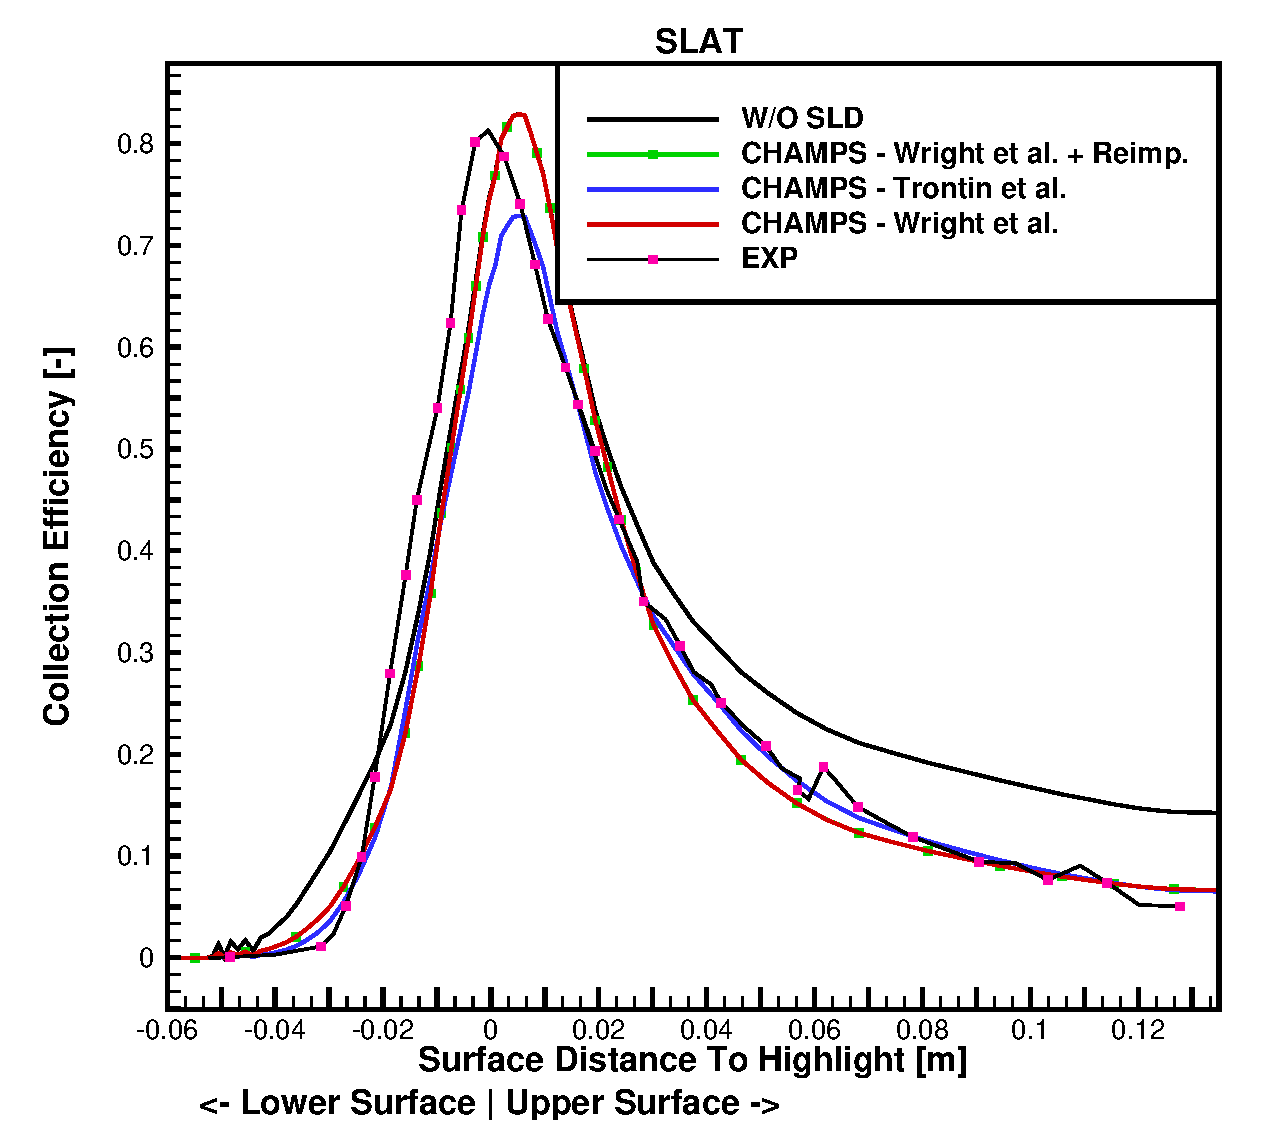
\includegraphics[width=\linewidth,height=3.3cm,keepaspectratio]{FIGURES/LAGRANGIAN/CASE_122_SLAT_SLD}\par\vspace{0.03cm}
    {\color{champsBlue}\bfseries\scriptsize SLAT}
  \end{column}
  \begin{column}{0.29\textwidth}
    \centering
    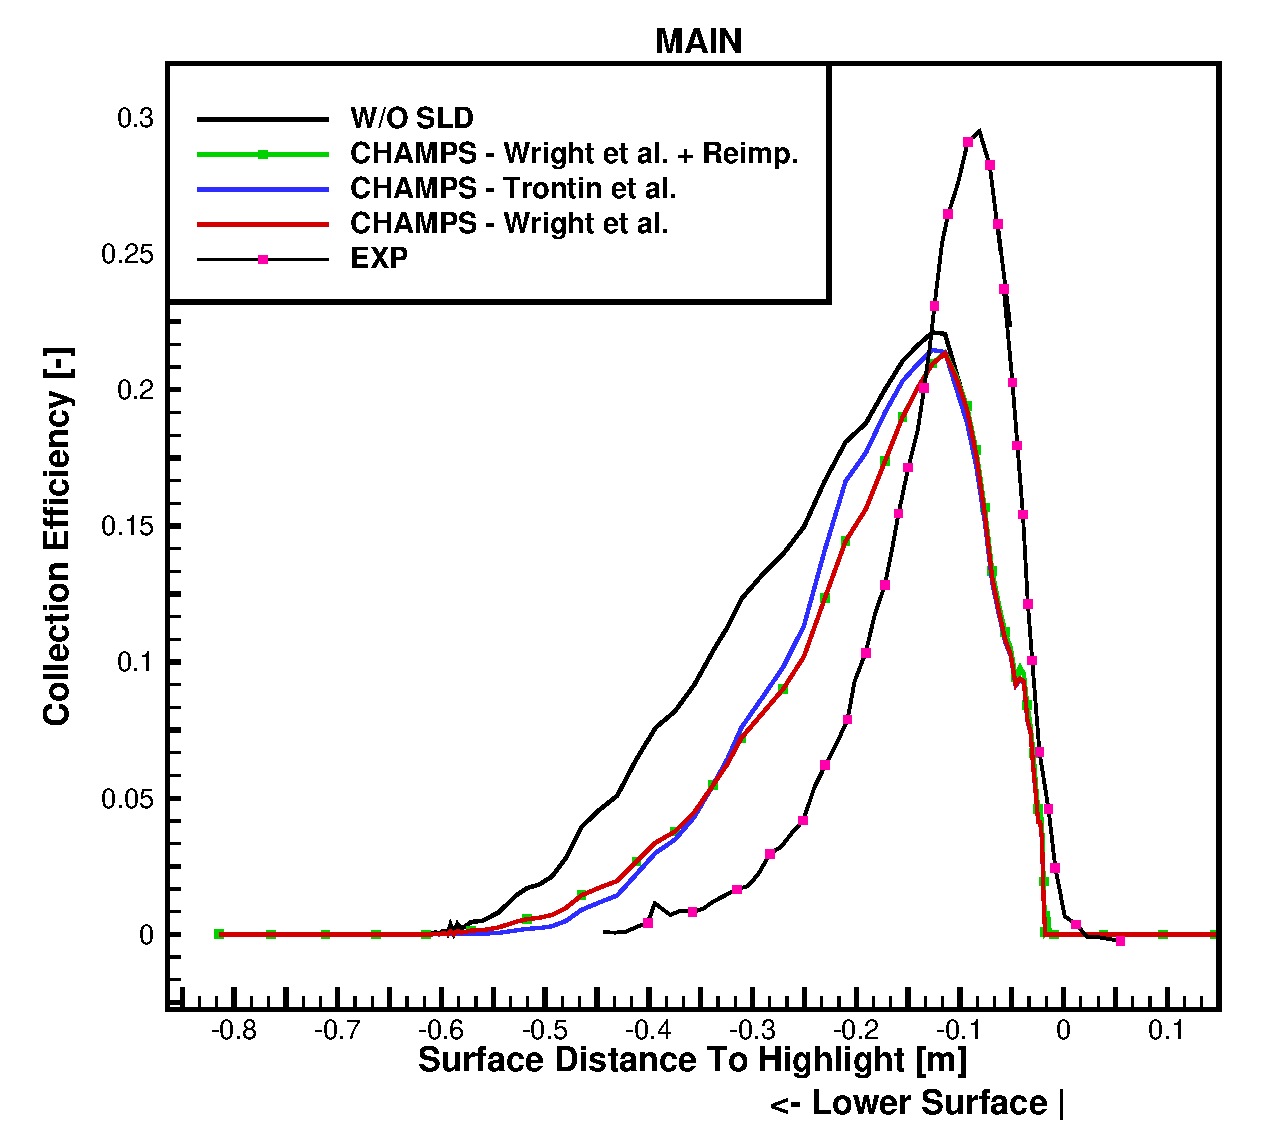
\includegraphics[width=\linewidth,height=3.3cm,keepaspectratio]{FIGURES/LAGRANGIAN/CASE_122_SLAT_MAIN}\par\vspace{0.03cm}
    {\color{champsBlue}\bfseries\scriptsize MAIN}
  \end{column}
  \begin{column}{0.29\textwidth}
    \centering
    \makebox[\linewidth][l]{\begin{tikzpicture}[spy using outlines={circle,magnification=1.9,size=1.85cm,connect spies,red,line width=0.8pt}]\node[inner sep=0,anchor=south west](im){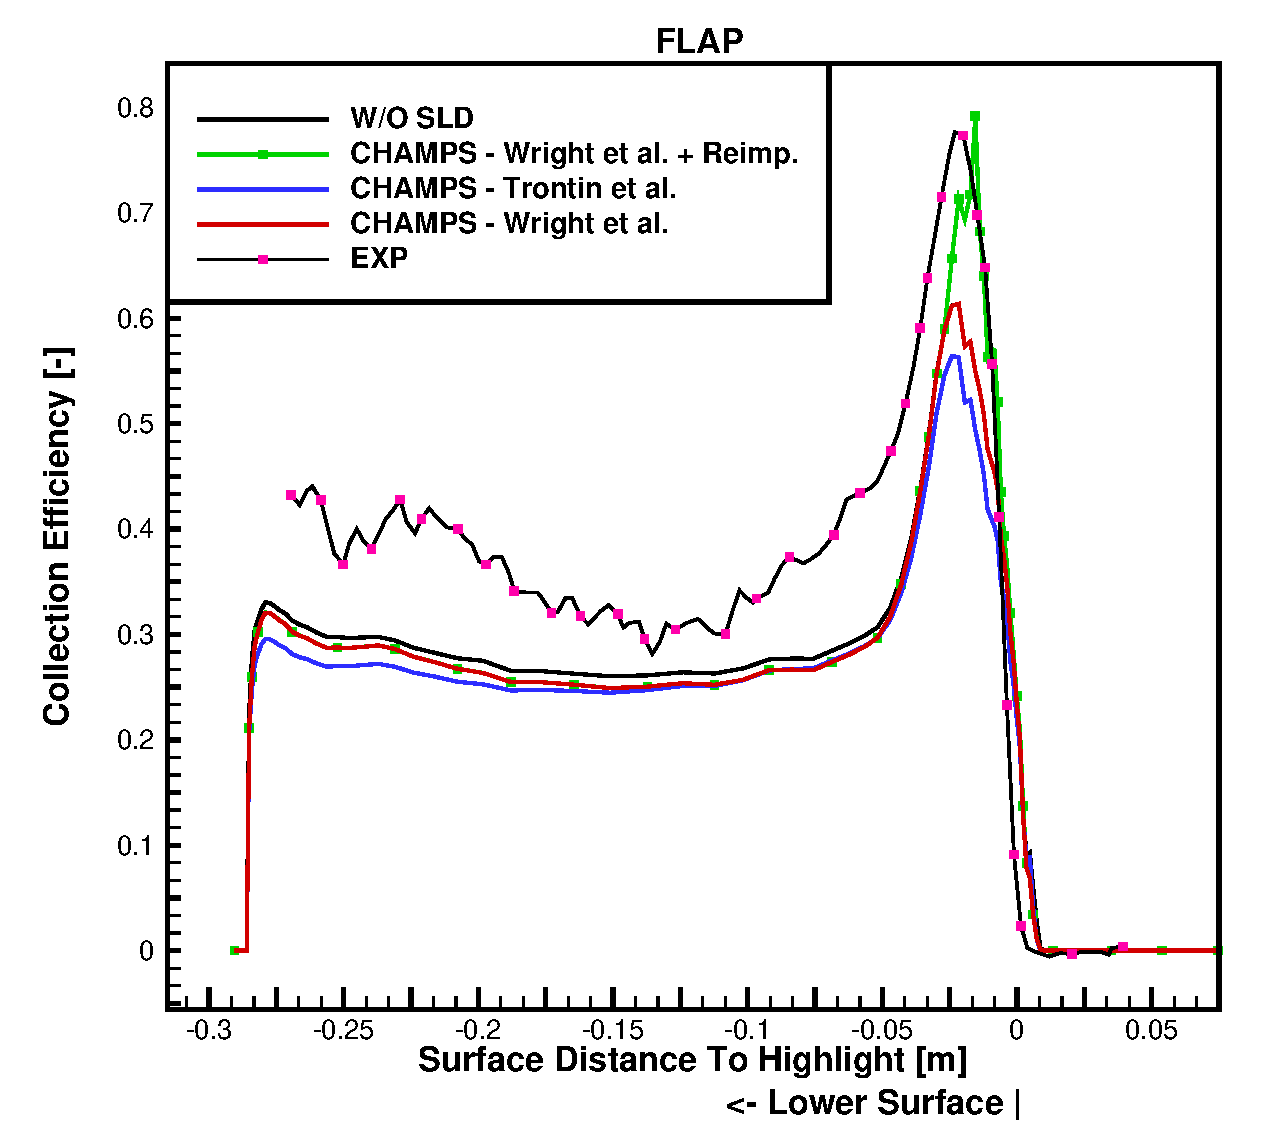
\includegraphics[width=\linewidth,height=3.3cm,keepaspectratio]{FIGURES/LAGRANGIAN/CASE_122_SLAT_FLAP}};\coordinate (pk) at ($0.772*(im.south east)+0.77*(im.north west)$);\coordinate (ln) at ($1.2*(im.south east)+0.5*(im.north west)$);\spy on (pk) in node at (ln);\end{tikzpicture}}\par\vspace{0.03cm}
    {\color{champsBlue}\bfseries\scriptsize FLAP}
  \end{column}
  \begin{column}{0.10\textwidth}\end{column}
\end{columns}
\vfill
\begin{center}
\begin{tikzpicture}
\node[fill=champsBlue!5, draw=champsBlue!18, rounded corners=4pt,
      text width=0.92\textwidth, inner sep=3pt, align=center, font=\small] {%
SLD models improve the $\beta$ prediction, especially on the slat, but not on the other elements, while reimpingement improves the flap peak.};
\end{tikzpicture}
\end{center}
\SlideRef{laurendeau2022summary}
\end{frame}

% Add section slides here.
